\documentclass[a4paper, notitlepage, 10pt]{article}
\usepackage{geometry}
% WSC 2015 configs
\fontfamily{times}
\geometry{verbose,tmargin=30mm,bmargin=25mm,lmargin=25mm,rmargin=25mm}
% end configs
\usepackage{setspace,relsize}               
\usepackage{moreverb}                        
\usepackage{url}
\usepackage{hyperref}
\hypersetup{colorlinks=true,citecolor=blue}
\usepackage{amsmath}
\usepackage{mathtools} 
\usepackage{amsthm}
\usepackage{amssymb}
\usepackage{indentfirst}
\usepackage{todonotes}
\usepackage{subfigure}
\usepackage{multirow}
\usepackage[authoryear,round]{natbib}
\bibliographystyle{apalike}
\usepackage[pdftex]{lscape}
\usepackage[utf8]{inputenc}
% Title Page
\title{\vspace{-9ex}\centering \bf On the choice of weights for the logarithmic pooling of probability distributions}
\author{
Luiz Max F. de Carvalho$^{a}$, Daniel A. M. Villela$^b$, Flavio Coelho$^a$ \& Leonardo S. Bastos$^b$ \\
a -- School of Applied Mathematics, Getulio Vargas Foundation (FGV)\\
b -- Program for Scientific Computing (PROCC), Oswaldo Cruz Foundation. \\
}
\DeclareMathOperator*{\argmin}{arg\,min}
\DeclareMathOperator*{\argmax}{arg\,max}
\newtheorem{theo}{Theorem}[]
\newtheorem{proposition}{Proposition}[]
\newtheorem{remark}{Remark}[]
\newtheorem{lemma}{Lemma}[]
\setcounter{theo}{0} % assign desired value to theorem counter
\begin{document}
\maketitle

\begin{abstract}
% Combining different prior distributions is an important issue in decision theory and Bayesian inference.
% Logarithmic pooling is a popular method to aggregate expert opinions by using a set of weights that reflect the reliability of each information source.
% The resulting pooled distribution however depends heavily on set of weights given to each opinion/prior.
% In this paper we explore% three
% approaches to assigning weights to opinions.
% Two methods are stated in terms of optimisation problems and a third one uses a hierarchical prior that accounts for uncertainty on the weights. 
% We explore several examples of interest, such as proportion and rate estimation and combining Normal distributions.
%TODO: more on the examples, make them prominent

% The Bayesian melding method concerns drawing inference about a deterministic model by combining a natural prior on quantities of interest (inputs and/or outputs) with the prior \textit{induced} by the model through logarithmic pooling.

Key-words: logarithmic pooling; expert opinion; hierarchical modelling; Bayesian melding. 
\end{abstract}

\section{Introduction}
\label{sec:intro}

Combining probability distributions is a topic of general interest, both in the statistical~\citep{West1984, Genest1986A, Genest1986B} and decision theory literatures~\citep{Genest1984,French1985,Guardoni2002}.
On the theoretical front, studying opinion pooling operators may give important insights on consensus belief formation and group decision making~\citep{West1984,Genest1986B,Guardoni2002}.
Among the various opinion pooling operators proposed in the literature, logarithmic pooling has enjoyed much popularity, mainly due to its many desirable properties such as relative propensity consistency (RPC) and external Bayesianity (EB)~\citep{Genest1986A} -- see below. 
In a practical setting, logarithmic pooling finds use in a range of fields, from engineering~\citep{Lind1988, Savchuk1994} to wildlife conservation~\citep{Poole2000} and infectious disease modelling~\citep{Coelho2009}. 

A common situation of interest is combining expert opinions about a quantity of interest $\theta \in \mathbf{\Theta} \subseteq \mathbb{R}^p$ when they can be represented as (proper) probability distributions.
Combining these opinions using logarithmic pooling requires assigning weights to each of the experts, which represent the (relative) reliability of each opinion~\citep{Genest1984}.
This requirement naturally leads to the question of how to choose the weights in a meaningful way, according to some well-accepted optimality criterion.
There are a few proposals in the literature that build methods using different approaches.
One proposal is to maximise the entropy the pooled distribution~\citep{Myung1996}, whereas another one is to minimise Kullback-Leibler (KL) divergence between the pooled distribution and the individual opinions~\citep{Abbas2009} or between the pooled (prior) distribution and the posterior distribution~\citep{Rufo2012A,Rufo2012B}.

These approaches, while moving away from the problem of arbitrarily assigning the weights, arrive at single point solutions, similar to point estimates in Statistical theory.
Albeit acknowledging that these approaches have merit, we argue that in many settings, where one has substantial prior information on the relative reliabilities of the information sources (experts), it would be desirable to incorporate this information into the pooling procedure while accommodating uncertainty about the weights.
Moreover, assigning a probability distribution over the weights allows one to obtain a posterior distribution using a Bayesian procedure, which in turn enables learning about the weights from data~\citep{Poole2000}.
Therefore, it makes possible to sequentially update knowledge about the reliability of each expert/source in the face of new data.

In this paper we discuss previous approaches for assigning the weights based on optimality criteria and study assigning hierarchical priors to the weights in order to learn about them from data.
This paper is organised as follows: in Section~\ref{sec:background} we introduce the necessary concepts and notation on logarithmic pooling, as well as some its key properties.
We also prove a new result about log-concavity of the pooled distribution when all distributions are log-concave.
In Section~\ref{sec:weights} we present different approaches to choose the weights, two methods based on optimality criteria, namely maximising the entropy of the pooled prior and minimising Kullback-Leibler divergence between the pooled distribution and the expert distributions.
In addition we also lay out an approach hierarchical modelling of the weights.
Section~\ref{sec:apps} contains applications of logarithmic pooling to reliability analysis (Sections~\ref{sec:survivalProbs} and~\ref{sec:learning_rate}), meta-analysis (Section~\ref{sec:metaAnalysis}) and Bayesian melding (Section~\ref{sec:melding_apps}).


\section{Logarithmic pooling: properties and applications}
\label{sec:background}

In this section we introduce the necessary theory and notation and motivate the use of the logarithmic pooling operator by presenting some of its desirable properties.

First let us define the logarithmic pooling (LP) operator.
Let $\mathbf{F}_{\theta} := \{f_0(\theta), f_1(\theta), f_2(\theta), \ldots, f_K(\theta)\}$ be a set of (densities of) prior distributions representing the opinions of $K+1$ experts and let $\boldsymbol\alpha :=\{\alpha_0, \alpha_1, \alpha_2, \ldots, \alpha_K \}$ be the vector of weights, such that $\alpha_i > 0\: \forall i$ and $\sum_{i=0}^K \alpha_i = 1$.
The log-pooled prior is
\begin{equation}
\label{eq:logpool}
 \mathcal{LP}(\mathbf{F_\theta}, \boldsymbol\alpha) := \pi(\theta \mid \boldsymbol\alpha) = t(\boldsymbol\alpha) \prod_{i=0}^K f_i(\theta)^{\alpha_i},
\end{equation}
where $t(\boldsymbol\alpha) = \left[ \int_{\boldsymbol\Theta}\prod_{i=0}^K f_i(\theta)^{\alpha_i}\, d\theta \right]^{-1}$.

Logarithmic pooling will only yield proper probability distributions if it is possible to normalise the expression in (\ref{eq:logpool}).
This condition is usually assumed implicitly, without proof.
While \citet{Poole2000} provide a proof for the case of two densities (see Theorem 1 therein),~\cite{Genest1986A} (pg.489) prove the result for a finite number of densities:
\begin{theo}
\label{thm:normalisation}
\textbf{Normalisation~\citep{Genest1986A}}. 
Let $A$ be a $(K+1)$-dimensional open simplex on $[0,1]$.
For all $\boldsymbol\alpha \in A$ there exists a constant $t(\boldsymbol\alpha)$ such that $\int_{\boldsymbol\Theta}\pi(\theta \mid \boldsymbol \alpha)\, d\theta = 1$.
\end{theo}
We give a simple proof using H\"{o}lder's inequality in the Appendix.
This result ensures any (finite) number of proper distributions can be combined using the logarithmic pooling operator to yield a normalisable (proper) density.
In addition, log-linear pools enjoy the~\textit{external Bayesianity} property (Remark~\ref{rmk:properties_EB}), which guarantees that whether one combines the expert opinions before or after observing evidence does not affect the resulting pooled distribution.
\begin{remark}
\label{rmk:properties_EB}
 \textbf{External Bayesianity~\citep{Genest1984}}.
 If the expert opinions are given by densities $f_i(\theta)$ and one observes data $x$ such that one can specify a likelihood $l(x \mid \theta)$, combining the set of posteriors $p_i(\theta \mid x) \propto  l(x \mid \theta)f_i(\theta) $ yields the same distribution as combining the densities $f_i$ to obtain a prior $\pi(\theta)$ and then combine it with $l(x \mid \theta)$ to obtain a posterior $p(\theta \mid x) \propto l(x \mid \theta)\pi(\theta)$.
\end{remark}
\begin{proof}
 The proof of this fact is trivial and is given here for completeness.
 Combining the posteriors $p_i(\cdot)$ gives
 \begin{align*}
  p^\prime (\theta \mid x, \boldsymbol \alpha) &\propto \prod_{i = 0}^K \left[  l(x \mid \theta)f_i(\theta) \right]^{\alpha_i},\\
  &\propto   l(x \mid \theta) \prod_{i = 0}^K f_i(\theta)^{\alpha_i},\\
  &=  \frac{l(x \mid \theta)\pi(\theta \mid \boldsymbol \alpha)}{m^{\prime}(x)} \equiv   p(\theta \mid x, \boldsymbol \alpha),
 \end{align*}
 where the second line follows from $\sum_{i=0}^K \alpha_i = 1$.
\end{proof}
Much less trivially,~\cite{Genest1984} show that the logarithmic pooling operator in~(\ref{eq:logpool}) is the~\textbf{only} aggregation (pooling) operator that enjoys external Bayesianity.
Moreover, the logarithmic pooling operator has the relative propensity consistency (RPC) property (Remark~\ref{rmk:properties_RPC}), whereby the pooled opinion preserves relative judgments from the experts.
\begin{remark}
\label{rmk:properties_RPC}
\textbf{Relative propensity consistency~\citep{Genest1984}}.
Taking $\boldsymbol F_{X}$ as a set of expert opinions with support on a space $\mathcal{X}$, define $\boldsymbol \xi = \{\boldsymbol F_{X}, a, b\}$ for arbitrary $a , b \in \mathcal{X}$.
Let $\mathcal{T}$ be a pooling operator and define two functions $U$ and $V$ such that 
\begin{align}
 U(\boldsymbol \xi) &:= \left( \frac{f_0(a)}{f_0(b)}, \frac{f_1(a)}{f_1(b)}, \ldots, \frac{f_K(a)}{f_K(b)} \right)\:\text{and}\\
 V(\boldsymbol \xi) & := \frac{\mathcal{T}_{\boldsymbol F_{X}} (a)}{\mathcal{T}_{\boldsymbol F_{X}} (b)}.
\end{align}
We then say that $\mathcal{T}$ enjoys \textit{relative propensity consistency} (RPC) if and only if
\begin{equation}
 U(\boldsymbol \xi_1) \geq U(\boldsymbol \xi_2) \implies  V(\boldsymbol \xi_1) \geq V(\boldsymbol \xi_2),
\end{equation}
for all $\boldsymbol \xi_1, \boldsymbol \xi_2$.
\end{remark}
We refer the reader to~\cite{Genest1984} for a proof.
Informally, this property says that if all experts consider a particular event $A$ more probable than another event $B$, then the pooled opinion should be consistent with these relative judgments. 
\cite{Genest1984} show that for mild conditions on $\mathcal{X}$, namely $|\mathcal{X}| \geq 3$, the logarithmic pooling operator is the only pooling operator with RPC (see also Lemma~\ref{lem:RPC_representation} in the Appendix).

Another desirable property of the logarithmic pooling operator is log-concavity.
Log-concavity of the pooled prior may be important to consider in order to guarantee unimodality and certain conditions on tail behaviour (see~\cite{Bagnoli2005}).
This motivates the following theorem, which is, to the best of our knowledge, a new result:
\begin{theo}
\label{thm:concavity}
\textbf{Log-concavity}. 
If $\mathbf{F}_{\theta}$ is a set of log-concave distributions, then $\pi(\theta\mid \boldsymbol \alpha)$ is also log-concave.
Moreover, logarithmic pooling is the~\underline{only} pooling operator that will always produce a log-concave density if all the elements of $\mathbf{F}_{\theta}$  are log-concave.
\end{theo}
\begin{proof}
 See the Appendix.
\end{proof} 
Theorem~\ref{thm:concavity} tells us that logarithmic pooling is the only aggregation method to universally preserve log-concavity, for any configuration of the weights ($\boldsymbol{\alpha}$).
This universality result is important because it holds for any set of log-concave distributions, $\mathbf{F}_{\theta}$.
In contrast, a linear pool of $K$ Gaussian distributions with common mean, for example, would produce a log-concave pooled distribution for any $\boldsymbol{\alpha}$, but this would fail if the means were different.

\subsection{Exponential family}
\label{sec:expofamily}

The exponential family of probability distributions finds widespread in the modelling of empirical phenomena.
In this section we give expressions for the entropy and Kullback-Leibler divergence for the pooled distributions. 
Suppose we are interested in a random variable, $Y$, from an exponential family with parameter $\theta$ and probability density function (pdf) given by
\begin{equation}
\label{eq:exponentialfamily}
f(y|\theta) = h(y) e^{\theta y - s(\theta)}.
\end{equation}

Let $\mathbf{F}_{y}$ be a set of densities on $y$ of the form in~(\ref{eq:exponentialfamily}), $f_i(y|\theta_i)$, $ i = 0, 1, \ldots, K$. 
The combined (log-pooled) distribution also belongs to the exponential family:
\begin{equation}
\label{eq:pooldistEF}
\pi(y| \boldsymbol\alpha ) = t(\boldsymbol\alpha) h^\ast (y) e^{\theta^\ast y - s^\ast (\boldsymbol\theta)},
\end{equation}
where $\boldsymbol\theta :=\{\theta_0, \theta_1, \ldots, \theta_K \}$, $h^\ast (y) = \prod_{i = 0}^K h_i(y)^{\alpha_i}$,  $\theta^\ast = \sum_{i = 0}^K \alpha_i \theta_i$ and $s^\ast (\boldsymbol\theta) = \sum_{i = 0}^K \alpha_i s_i(\theta_i)$.

The entropy function of the log-pooled distribution is
\begin{equation}
\label{eq:entropydistEF}
H_\pi(Y; \boldsymbol\alpha) :=  - \mathbb{E}_{\pi}\left[-\log \pi(Y | \boldsymbol\alpha) \right] = -\log t(\boldsymbol\alpha) + s^\ast (\boldsymbol\theta) - \mathbb{E}_\pi[\log h^\ast (Y)] - \theta^\ast \mathbb{E}_\pi[Y] \: ,
\end{equation}
where $\mathbb{E}_{\pi}\left[ g(Y) \right]$ is the expectation of a $\pi$-measurable function $g(Y)$ with respect to $\pi( y | \boldsymbol\alpha)$, when the integral exists.

The Kullback-Leibler divergence between the pooled distribution (\ref{eq:pooldistEF}) and each distribution in $\mathbf{F}_{y}$ can be written as:
\begin{equation}
\label{eq:KLdistEF}
KL(\pi || f_i )  =  - H_\pi(Y; \boldsymbol\alpha) - \mathbb{E}_\pi[\log h_i(Y)] - \theta_i \mathbb{E}_\pi[Y] + s_i(\theta_i).
\end{equation}

These expressions allow for easy computation of information measures for a broad class of distributions, which will be useful in the remainder of this paper (see also the Appendix).

\subsubsection{Conjugate priors to the exponential family}
\label{sec:conjugexpofamily}

A conjugate prior family for $f(y|\theta)$ (\ref{eq:exponentialfamily}), has the following form~\citep{Diaconis1979}:
\begin{equation}
\label{eq:priorEF}
g(\theta | a, b) = K(a,b) e^{\theta a - b s(\theta)} \: ,
\end{equation}
where $K(a,b)$ is a normalising constant.
Similar to the above, let $\mathbf{G}_{\theta}$ be a set of log-conjugate prior distributions representing the opinions of $K+1$ experts, and $g_i(\theta) = g(\theta | a_i, b_i)$ from equation (\ref{eq:priorEF}).

The log-pooled prior is also a conjugate prior for $f(y|\theta)$ with hyperparameters given by a weighted mean of the experts hyperparameters, i.e., $\pi(\theta|\boldsymbol\alpha) = g(\theta | a^*, b^* )$, where $a^* = \sum_{i=0}^K \alpha_i a_i$ and $b^* = \sum_{i=0}^K \alpha_i b_i$.
% \begin{equation}
% \label{eq:poolpriorEF}
% \pi(\theta|\boldsymbol\alpha) = g(\theta | a^*, b^*) \: ,
% \end{equation}
% where $a^* = \sum_{i} \alpha_i a_i$ and $b^* = \sum_{i} \alpha_i b_i$.
% Note that the posterior distribution of $\theta$ is given by $\pi(\theta | y) = g(\theta | a^* + y, b^* + 1)$.

The entropy function of the log-pooled prior (\ref{eq:priorEF}) is given by
\begin{equation}
\label{eq:entropypriorEF}
H_\pi(\theta; \boldsymbol\alpha) = - \log (K(a^*, b^*))  -  a^*  \mathbb{E}_\pi[\theta]  +  b^*  \mathbb{E}_\pi[s(\theta)] \: .
\end{equation}

And the Kullback-Leibler divergence, $KL(\pi || g_i )$, is the following
\begin{equation}
\label{eq:KLpriorEF}
KL( \pi || g_i ) = - H_\pi(\theta; \boldsymbol\alpha) - \log( K(a_i,b_i)) - a_i \mathbb{E}_\pi[\theta] + b_i \mathbb{E}_\pi[s(\theta)] \: .
\end{equation}


\subsection{Bayesian melding}
\label{sec:background_melding}

Another important application of logarithmic pooling is in the Bayesian melding method of~\cite{Poole2000}.
Deterministic simulation models are widespread in Science and Engineering (see~\cite{Poole2000} and references therein).
One is often interested in a deterministic model $M$ with inputs $\theta \in \boldsymbol\Theta \subseteq \mathbb{R}^p$ and outputs $\phi \in \boldsymbol\Phi\subseteq \mathbb{R}^q$, such that $\phi = M(\theta)$.
If one wants to learn about $\theta$ from data and a (prior) distribution on $\phi$ is available, then one needs a method to combine the information between the prior on $\theta$ and the prior induced on it  through $M$, which is often non-invertible.

Bayesian melding seeks to draw inference by first employing logarithmic pooling to construct a prior on $\phi$ of the form
\begin{equation}
 \label{eq:BMpoolprior}
 \tilde{q}_{\Phi}(\phi) \propto q_1^\ast(\phi)^\alpha q_2(\phi)^{1-\alpha},
\end{equation}
where $q_1^\ast()$ is the \textbf{induced} prior on the outputs and $q_2$ is the prior on $\phi$ without considering the deterministic model, henceforth called the natural prior on $\phi$.
The prior in~(\ref{eq:BMpoolprior}) can then be inverted to obtain a \textit{coherised} prior on $\theta$, $\tilde{q}_{\Theta}(\theta)$.
\cite{Poole2000} give  a way of obtaining $\tilde{q}_{\Theta}$ even when $M$ is non-invertible, which we will not discuss further here. 

Standard Bayesian inference may then follow,  leading to the posterior
\begin{equation}
 \label{eq:BMpoolposterior}
 p_{\Theta}(\theta) \propto \tilde{q}_{\Theta}(\theta) L_1(\theta) L_2(M(\theta)),
\end{equation}
which enjoys all the properties of usual posterior distributions.
The method allows standard Bayesian inference to be carried out about all quantities of interest in the model, which makes it attractive to application in policy making~\citep{Alkema2008}, where proper acknowledgement of uncertainty is crucial.

In~\cite{Poole2000} (Section 6.2), the authors fix $\alpha = 1/2$, justifying their choice by the fact that while the weights should reflect the reliability of each expert (information source), in the case of their Bayesian melding analysis one is combining distributions based on different bodies of evidence, but assessed by the same expert.
Since this need not be the case in all applications, in this paper we relax this restriction, modelling $\alpha$ through a hyperprior instead. 

\section{Assigning the weights in logarithmic pooling}
\label{sec:weights}

The weights, $\boldsymbol \alpha$, play a key role on the logarithmic pooling and hence their choice is critical.
Building on work by~\cite{Poole2000,Rufo2012A,Rufo2012B} and~\cite{Abbas2009}, we now move on to study three approaches to assigning the weights in logarithmic pooling.
The first two approaches are based on optimality criteria and a third method proposes assigning a (hyper)prior to the weights.

\subsection{Choosing weights based on optimality criteria}

\subsubsection{Maximising entropy}
\label{sec:maxent}

In a context of near complete uncertainty about the relative reliabilities of the experts (information sources) it may be desirable to combine the prior distributions such that $\pi(\theta)$ is maximally uninformative. %% LM: this can be highly problematic...
Such approach would ensure that, given the constraints imposed by $\mathbf{F}_{\theta}$, the pooled distribution is the one which best represents the current state of knowledge~\citep{Jaynes1957,Savchuk1994}.
In order to choose $\boldsymbol\alpha$ so as to maximise prior 
diffuseness, one can maximise the entropy of the log-pooled prior, i.e.
\begin{align}
\nonumber
H_{\pi}(\theta; \boldsymbol\alpha) &= E_{\pi}\left[-\log \pi(\theta) \right] =-\int_{\boldsymbol\Theta}\pi(\theta)\log\pi(\theta)\, d\theta,\\
\label{eq:entropypiB}
&= -\sum_{i=0}^{K} \alpha_i E_{\pi}[\log f_i] - \log t(\boldsymbol\alpha).
\end{align}
Formally, we want to find $\hat{\boldsymbol\alpha}$ such that
\begin{equation}
\label{eq:argmaxEnt}
 \hat{\boldsymbol\alpha}:= \argmax_{\boldsymbol\alpha} H_{\pi}(\theta; \boldsymbol\alpha).
\end{equation}

This approach, however, does not result in a convex optimisation problem, therefore one is not guaranteed to find a unique solution -- see Remark~\ref{rmk:uniqueness} for intuition as to why.

\subsubsection{Minimising Kullback-Leibler divergence}
\label{sec:minKL}

One could also wish to choose the pooling weights so as to minimise the total Kullback-Leibler divergence between the pooled distribution, $\pi$, and each distribution in $\mathbf{F}_{\theta}$.
Let $E_i[g]$ be the expectation of a measurable function $g: \boldsymbol{\Theta} \to \mathbb{R}$ with respect to each density $f_i$.
We can define a loss function such that
\begin{align}
\nonumber
L(\boldsymbol\alpha) &= \sum_{i=0}^K  \text{KL}(f_i || \pi ), \\
\label{eq:KLexpanded}
     &= - (K+1)\log t(\boldsymbol\alpha) - (K+1) \sum_{i=0}^K\alpha_i E_i [\log f_i ]  + \sum_{i=0}^K \mathbb{E}_i\left[\log f_i\right], 
\end{align}
and we want to find 
\begin{equation}
\label{eq:argminKL}
    \hat{\boldsymbol\alpha}:= \:\argmin_{\boldsymbol\alpha} L(\boldsymbol\alpha).   
\end{equation}
Fortunately, this set up leads to a unique solution, a result we summarise in Remark~\ref{rmk:uniqueness}.
\begin{remark}
\label{rmk:uniqueness}
\textbf{Uniqueness} .
 The distribution obtained following~(\ref{eq:argminKL}) is unique, i.e., there is only one aggregated prior $\pi(\theta \mid \boldsymbol\alpha)$ that minimizes $L(\boldsymbol\alpha)$.
\end{remark}
\begin{proof}
We begin by noting that the second term in~(\ref{eq:KLexpanded}) is a linear combinations of the weights, and hence we may restrict attention only to the first term -- the third term does not depend on $\boldsymbol{\alpha}$.
Next, recall that minimising~(\ref{eq:KLexpanded}) is equivalent to maximising $\log t(\boldsymbol\alpha) = \log\int_{\boldsymbol\Theta}\prod_{i=0}^{K}f_i(\theta)^{\alpha_i}\, d\theta$.
Proposition 3.1 in~\cite{Rufo2012A} states that $t(\boldsymbol\alpha)$ is log-concave, therefore any optimisation problem which involves minimising $-\log t(\boldsymbol{\alpha})$ is convex.
We thus conclude that the problem in~(\ref{eq:argminKL}) has a unique solution.
\end{proof}
By contrast, the problem in~(\ref{eq:argmaxEnt}) requires one to minimise $\ln t(\boldsymbol\alpha)$, hence lacking a sufficient condition for the existence of a unique solution.
Likewise, using  the loss function $L^\prime(\boldsymbol\alpha) = \sum_{i=0}^K  \text{KL}(\pi ||f_i )$ would not lead to a unique solution.
See Section~\ref{sec:computation_opt} for implementation details.

\subsection{Hierarchical modelling of the weights}
\label{sec:hierPrior}

As discussed by~\cite{Poole2000} and others~\citep{Zhong2015,Li2017}, estimating the weights would be of interest since this would allow one to assess the reliability of each source of information (expert).
\cite{Li2017} explore the idea of computing the pooled distribution for several values of the weights.
Whilst informative, this approach has two issues: (a) it does not scale well with increasing the number of distributions being combined, $K$, and; (b) it fails to account for any (posterior) dependence between model parameters and the weights.
In this section we propose placing a hierarchical prior on the weights, allowing for standard Bayesian inference on these quantities.

A natural choice for a prior distribution for $\boldsymbol\alpha$ is the $(K+1)-$dimensional Dirichlet distribution
\begin{equation}
 \label{eq:generalcondprior}
 \pi_A(\boldsymbol\alpha) = \frac{1}{\mathcal{B}(\boldsymbol x)}\prod_{i=0}^K \alpha_i^{x_i-1},
\end{equation}
where $\boldsymbol x = \{ x_0, x_1, \ldots, x_K\}$ is the vector of hyperparameters for the Dirichlet prior and $\mathcal{B}(X)$ is the multinomial beta function.
The Dirichlet offers a simple, albeit potentially inflexible prior.

A more flexible prior for $\boldsymbol\alpha$ is the logistic-normal distribution~\citep{Aitchson1980}:
\begin{equation}
 \label{eq:aitchinsonprior}
 \pi_A(\boldsymbol\alpha \mid \boldsymbol \mu, \boldsymbol \Sigma) = \frac{1}{|2\pi \boldsymbol \Sigma|^{\frac{1}{2}}}\frac{1}{\prod_{i=0}^K \alpha_i}
  \exp\left(
     \left(\log\left(\frac{\boldsymbol \alpha_{-K}}{\alpha_K}\right) - \boldsymbol \mu\right)^T
     {\boldsymbol \Sigma}^{-1}
     \left(\log\left(\frac{\boldsymbol \alpha_{-K}}{\alpha_K}\right) - \boldsymbol \mu\right)
     \right),
\end{equation}
where $\boldsymbol \alpha_{-K}$ represents the vector $\boldsymbol \alpha$ without the $K$-th element, $\boldsymbol \mu$ is a $K$-size mean vector, and $\boldsymbol \Sigma$ is a $K \times K$ covariance matrix.
\citep{Aitchson1980} propose choosing $\boldsymbol \mu$ and $\boldsymbol \Sigma$ minimizing the KL divergence between the Dirichlet (\ref{eq:generalcondprior}) and the logistic-normal (\ref{eq:aitchinsonprior}) distributions, i.e.
\begin{align}
 \label{eq:momentmatching}
 \mu_i & = \psi(x_i) - \psi(x_K), \quad i=0,1,\ldots,K-1, \\
 \Sigma_{ii} & = \psi'(x_i) + \psi'(x_K), \quad i=0,1,\ldots,K-1, \\
 \Sigma_{ij} & = \psi'(x_K),
\end{align}
where $\psi(\cdot)$ is the digamma function, and $\psi'(\cdot)$ is the trigamma function.

The marginal prior for $\theta$,
\begin{equation}
\label{eq:marginalbeta}
\pi(\theta) = \int_{\mathcal{A}} \pi(\theta \mid \boldsymbol\alpha) \pi_A(\boldsymbol\alpha)d\boldsymbol\alpha,
\end{equation}
can also be efficiently approximated through Monte Carlo sampling when $\pi$ can be written in closed-form.
Even when it cannot be expressed analytically, it is still possible to sample from the marginal prior by using quadrature-based methods for computing $t(\boldsymbol\alpha)$ when $\theta$ is unidimensional (see Discussion).

\subsection{Computational details}
\label{sec:computation}

The analyses presented in this paper necessitated numerical optimisation to find the weights based on optimality criteria and Markov chain Monte Carlo (MCMC) to approximate posterior distributions.
All computations were carried out in the R~\citep{R2019} statistical computing environment, version 3.6.0. 
We provide implementations using the Stan~\citep{Carpenter2017} probabilistic programming language and R code for the methods, figures and tables presented in this paper can also be found at~\url{https://github.com/maxbiostat/opinion_pooling}.

\subsubsection{Optimisation procedures}
\label{sec:computation_opt}

In this section we give more detail on the optimisation procedures used to solve the problems in Sections~\ref{sec:maxent} and~\ref{sec:minKL}.
Since both problems are numerically unstable, we employ an strategy that starts the optimisation routine from $J = 1000$ overdispersed points in the unconstrained space, $\mathbb{R}^K$, obtained through the unit simplex transform~\citep{Betancourt2012}.
The procedure then picks the overall lowest/highest optimised value in order to avoid local minima/maxima.
We draw the initial values from a normal distribution with mean $0$ and variance $100^2$ and then employ the \verb|optim()| function to optimise the target functions (maximum entropy or minimum KL) using the L-BFGS algorithm~\citep{Byrd1995} with default settings.
We then choose the minimum/maximum achieved over the $J$ starting points in order to improve the chances of achieving a global optimum.

\subsubsection{Markov chain Monte Carlo \textit{via} Stan}
\label{sec:computation_mcmc}

Most of the posterior distributions discussed in this paper cannot be computed in closed-form and therefore we resort to Hamiltonian Monte Carlo~\citep{Neal2011}, in particular the No-U-Turn (NUTS) dynamic implementations available in Stan~\citep{Hoffman2014,Betancourt2017}.

For most computations, we employed four independent chains of $4000$ iterations each with the first $2000$ discarded as warm-up/burn-in.
Some models presented more challenging target distributions and we increased the number of iterations to $10 000$.
For all results reported, Monte Carlo error (MCSE) was well below 1\% the posterior standard deviation for all parameters, allowing for accurate computation of the relevant expectations.
In order to cope with challenging posterior geometry and ensure accurate computation, we used an acceptance probability of $0.99$ (\verb|adapt_delta = 0.99|, in Stan parlance) and up to $2^{15}$ leapfrog steps (\verb|max_treedepth = 15|).
All potential scale reduction factors ($\hat{R}$, \cite{Gelman1992}) were below $1.01$, indicating no convergence problems.

\subsubsection{Sampling-importance-resampling}
\label{sec:spIR}

In the context of Bayesian melding, while it is possible to employ HMC, it is sometimes preferable to employ custom algorithms that can better deal with the constraints imposed by the deterministic model.
In the original paper,~\cite[sec. 3.4]{Poole2000} propose a sampling-importance-resampling (SpIR) algorithm to sample from the posterior in~(\ref{eq:BMpoolposterior}), which we extend here to in order to accommodate varying weights.
\begin{enumerate}
\setcounter{enumi}{-1}
 \item Draw $k$ values from  $q_1(\theta)$, constructing $\boldsymbol \theta_k = (\theta^{(1)}, \theta^{(2)}, \ldots, \theta^{(k)} )$;
 \item Similarly, sample $\boldsymbol \alpha_k$ from $\pi(\boldsymbol \alpha)$;
 \item For each $\theta^{(i)} \in \boldsymbol\theta_k$ run the model to compute $\psi^{(i)} = M(\theta^{(i)})$, constructing $\boldsymbol \phi_k$;
 \item Obtain a density estimate of $q_1^\star(\phi)$ from  $\boldsymbol \phi_k$;
 \item Form the importance weights 
 \begin{equation}
 \label{eq:SpIRweights}
  w_i = t\left(\boldsymbol \alpha^{(i)}\right) \left(\frac{q_2(M(\theta^{(i)}))}{q_1^\star(M(\theta^{(i)}))}\right)^{1 - \boldsymbol \alpha^{(i)}} L_1(\theta^{(i)}) L_2(M(\theta^{(i)})),
 \end{equation}
where $t\left(\boldsymbol \alpha^{(i)}\right) = \left( \int_{\Phi} q_1^\ast(\phi)^{\alpha^{(i)}} q_2(\phi)^{1-\alpha^{(i)}} d\phi \right)^{-1}$ is computed using standard quadrature methods;
 \item (Re)Sample $l$ values from $\boldsymbol \theta_k$ according to the weights $\boldsymbol w_k$.
\end{enumerate}
The quadrature-based normalisation in step in 4 can be replaced with an importance sampling or MCMC estimate when the dimension of $\phi$ or $\theta$ is bigger than 1, but this is not explored here.

\section{Applications}
\label{sec:apps}

\subsection{Elicitation: combining expert priors on survival probabilities}
\label{sec:survivalProbs}

The first example we consider is combining expert opinions about probabilities and proportions.
We analyse an example proposed by~\cite{Savchuk1994} (also discussed in~\cite{Rufo2012B}) in which four experts are required supply prior information about the survival probability $\theta$ of a certain unit.
The experts express their opinion as prior means for the survival probability, which~\cite{Savchuk1994} then use to construct prior distributions with maximum variance given the restriction on the means.
From the vector of prior means $\mathbf{m} = \{ m_0 = 0.95, m_1 = 0.80, m_2 = 0.90, m_3 = 0.70 \}$, the authors obtain the parameters of the Beta distributions for each expert,  $\mathbf{a} = \{ a_0 = 18.10, a_1 = 3.44 , a_2 = 8.32, a_3 = 1.98 \}$ and  $\mathbf{b} = \{ b_0 = 0.955 , b_1 = 0.860, b_2 = 0.924, b_3 = 0.848\}$.
Furthermore, an experiment is conducted and $y = 9$ successes out of $n = 10$ trials are observed.
Thus, in this application we are able to estimate the posterior distribution for the survival probability and also, with  the hierarchical modelling approach, the posterior distribution for the weights in face of the observed data.
For the hierarchical priors, we employ a $\text{Dirichlet}(1/10, 1/10, 1/10, 1/10)$ and a moment-matching logistic-normal priors (see Section~\ref{sec:learning_rate} for a justification).

The probability density of the survival probability for each expert is given by
$$f_i(\theta;a_i, b_i) = \frac{1}{\mathcal{B}(a_i, b_i)} \theta^{a_i-1}(1-\theta)^{b_i-1},$$
where $\mathcal{B}(a,b)= \Gamma(a)\Gamma(b)/\Gamma(a + b)$ is the Beta function.
The log-pooled distribution for $\theta$ is then
\begin{align}
\nonumber
\pi(\theta) & = t(\boldsymbol\alpha)\prod_{i=0}^{K}f_i(\theta;a_i,b_i)^{\alpha_i},\\
\nonumber
            & \propto \prod_{i=0}^{K} \left(\theta^{a_i-1}(1-\theta)^{b_i-1} \right)^{\alpha_i},\\
\label{eq:betabern}
&\propto \theta^{a^*-1}(1-\theta)^{b^*-1},
\end{align}
with $a^* =\sum_{i=0}^{K}\alpha_ia_i$ and $b^* = \sum_{i=0}^{K}\alpha_ib_i$.
Note that (\ref{eq:betabern}) is the kernel of a Beta distribution with parameters $a^*$ and $b^*$. Hence the entropy is the following
\begin{equation}
 \label{eq:entropybeta}
 H_{\pi}(\theta) = \log \mathcal{B}(a^*,b^*) - (a^*-1)\psi(a^*) - (b^*-1)\psi(b^*) + (a^*+b^* -2)\psi(a^*+b^*).
\end{equation}
And the KL divergence between $\pi(\theta)$ and $f_i(\theta)$  is
\begin{equation}
\begin{split}
 \label{eq:KLbeta}
 d_i = KL(\pi || f_i) = \ln\left(\frac{\mathcal{B}(a_i, b_i)}{\mathcal{B}(a^*, 
b^*)}\right) & + (a^* - a_i) \psi(a^*)+ (b^* - b_i)\psi(b^*) \\
 &- (a^*-a_i + b^* - b_i)\psi(a^*+b^*).
\end{split}
\end{equation}

Table~\ref{tab:alphasBeta} lists the weights proposed by the methods discussed above, as well as the solution found by~\cite{Rufo2012B} (Section 5.2).
We note that the weights from maximum entropy, minimum KL divergence and using the method by~\cite{Rufo2012B} use only information contained in the collection of expert distributions $\boldsymbol F_{\theta}$, while the results for the hierarchical priors are posterior means obtained after observing data.
Maximising the entropy of the pooled distribution lead to the degenerate solution $\boldsymbol \alpha = \{0, 0, 0, 1 \}$, which gives all the weight to the most diffuse prior distribution -- $\text{Beta}(1.98, 0.848)$.
Since $t(\boldsymbol\alpha)$ is concave, we expect to find the maximum entropy given by the boundary conditions, which may lead to points in the border of the simplex.
Unsurprisingly, the same solution was found by~\cite{Rufo2012B} whose method tends to favour more diffuse distributions.
Minimising Kullback-Leibler divergence between the pooled prior and each expert prior leads to a unique solution but in this case also suggests to discard two of the opinions.
The hierarchical priors gave very similar posterior distributions for the weights, which assign the experts nearly equal weights.

\begin{table}[ht]
\caption{\textbf{Weights obtained using different methods for the survival probability example~\citep{Savchuk1994}.}
$^1$ -- Kullback-Leibler; $^2$ -- Posterior mean for $\boldsymbol\alpha$.}
\centering
\begin{tabular}{ccccc}
  \hline
Method  & $\alpha_0$ & $\alpha_1$ & $\alpha_2$ & $\alpha_3$ \\ 
  \hline
Maximum entropy & 0.00 & 0.00 & 0.00 & 1.00 \\ 
Minimum KL$^1$ divergence & 0.04 & 0.96 & 0.00 & 0.00 \\
\cite{Rufo2012A} & 0.00 & 0.00 & 0.00& 1.00\\
Dirichlet prior$^2$ & 0.26 & 0.24 & 0.27 & 0.23 \\ 
Logistic-normal prior$^2$ & 0.27 & 0.24 & 0.31 & 0.18\\
 \hline
\end{tabular}
\label{tab:alphasBeta}
\end{table}

Figure~\ref{fig:priors_pooled_Savchuk} shows the prior densities for each expert and pooling method and Table~\ref{tab:prior_posteriorsSavchuk} contains the prior and posterior mean and credibility intervals from each of the methods and also the case in which we assign an equal weight ($1/K$) to each opinion.
Assigning equal weights actually gives a prior mean that is the same as the maximum likelihood estimate of $\theta$, $\hat{\theta} = 9/ 10$.
This explains why both hierarchical posteriors resemble equal weights so closely.
Finally, we use the integrated (marginal) likelihood (\cite{Raftery2007}, eq. 9), $l(y) = \int_{0}^{1}f(y|\theta)\pi(\theta)\, d\theta$, as a univariate summary to compare the priors.
The marginal likelihood for the $i$-th expert and $J$ observations of the form $\{ y_j, n_j\}$ is:
\begin{align}
  \label{eq:marglike}
l_i(y_j, n_j) &= \int_{0}^{1}\mathcal{L}(\theta|y_j, n_j)\pi_i(\theta)\, d\theta\nonumber\\
 &= \prod_{j = 1}^{J}\frac{\Gamma(n_j-1)}{\Gamma(n_j-y_j + 1)\Gamma(y_j+1)}\frac{\Gamma(a_i + b_i)}{\Gamma(a_i + b_i + n_j)}\frac{\Gamma(a_i + y_j)}{\Gamma(a_i)}\frac{\Gamma(b_i + n_j - y_j) }{\Gamma(b_i)}.
 \end{align}
For the hierarchical priors we take the posterior mean of $(a^\star, b^\star)$ as $(a_i, b_i)$.
Results are given in Table~\ref{tab:marglikes} and show that, apart from expert $3$ -- and hence the maximum entropy pooled prior--, all other pooled priors and individual experts' priors give similar marginal likelihoods.
If one were to normalise the marginal likelihoods in order to form the expert weights, one would find $\boldsymbol\alpha^\prime = \{0.27, 0.24, 0.30, 0.19 \}$, which is not very different from equal weights.
The posterior distribution for the weights estimated under both priors favours expert 1, the expert with the highest marginal likelihood.
The logistic-normal gives expert 1 a higher weight when compared with the Dirichlet.
This is connected to the increased flexibility of the logistic-normal (see Section~\ref{sec:learning_rate}).

We stress that that the marginal likelihoods are not being used here as a means of selecting priors, but rather as a useful univariate summary that is informative about the compatibility with the observed data and hence informative about prior-data conflict.
While in this example one can gain insight into prior-data conflict from just the prior means and $y/n$, in other situations it might be harder to discern which expert gave the best (prior) guess, for instance.
% In section~\ref{sec:learning_rate} we address the issue of the performance of both prior hierarchical priors and how one can update the weights  

\begin{figure}[!ht]
\begin{center}
\subfigure[][Expert priors]{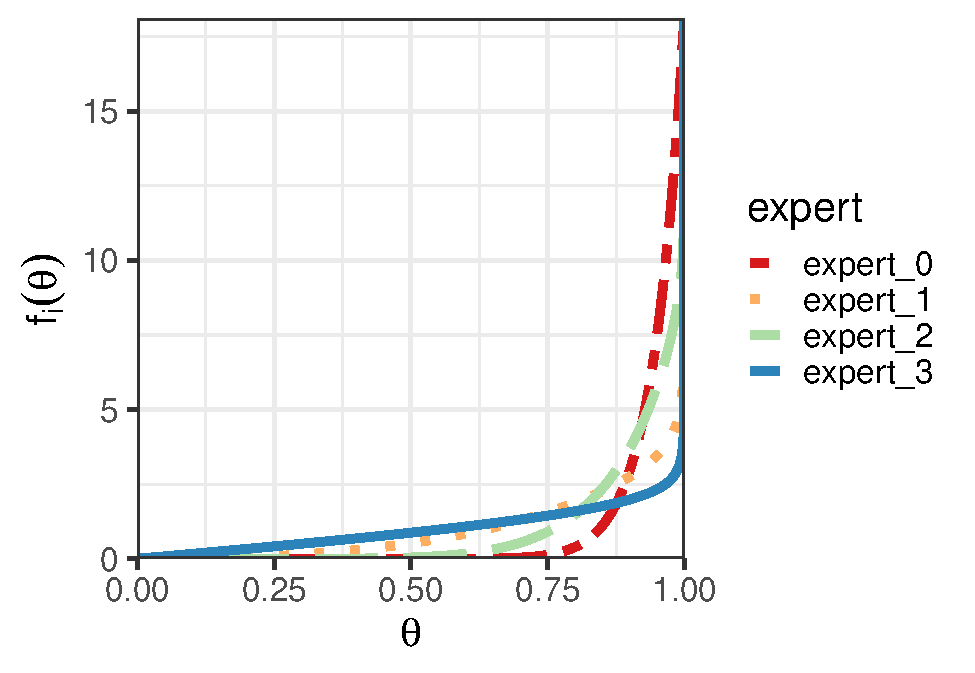
\includegraphics[scale=.35]{../plots/expert_densities_Savchuk.pdf}}
\subfigure[][Pooled priors]{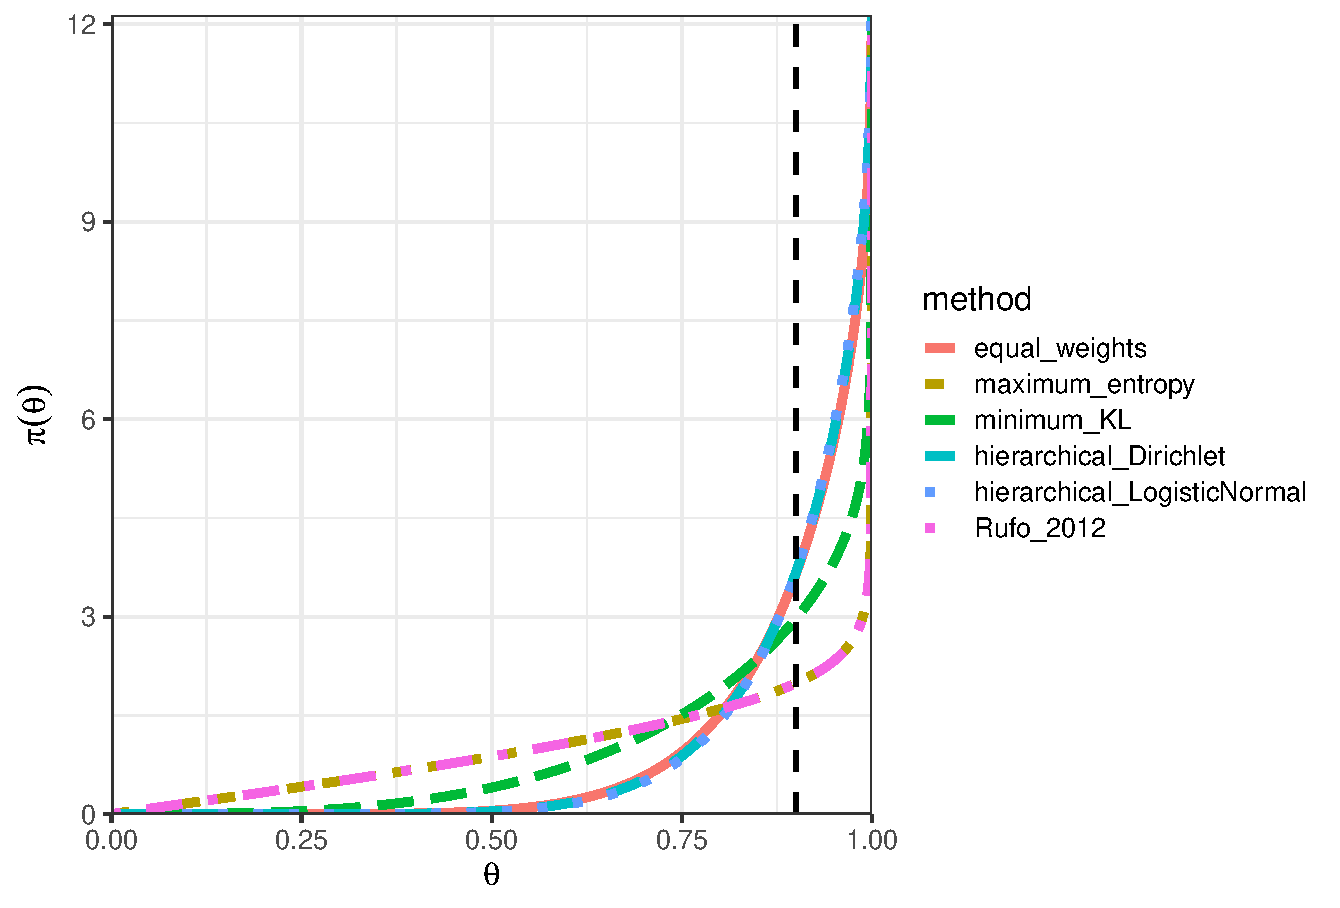
\includegraphics[scale=.35]{../plots/method_prior_densities_Savchuk.pdf}}
\end{center}
\caption{\textbf{Prior and posterior densities for the survival probability $\theta$}.
Panel (a) shows the distributions elicited by each expert (data from~\cite{Savchuk1994}) and panel (b) shows the pooled priors and posteriors obtained using the methods discussed in this paper and the solution found by~\cite{Rufo2012B}.
The black dashed vertical line marks the maximum likelihood estimate of $\theta$, $\hat{\theta}= 9/10$.
}
\label{fig:priors_pooled_Savchuk}
\end{figure}

\begin{table}[ht]
\caption{\textbf{Prior and posterior mean and credibility intervals for each method for assigning the weight, survival probability example~\citep{Savchuk1994}.}
Values for the hierarchical priors are from the marginal prior of $\theta$ in~(\ref{eq:marginalbeta}).
}
\centering
\begin{tabular}{ccc}
 \hline
Method & Prior & Posterior  \\ 
 \hline
 Equal weights & 0.90 (0.64--1.00) & 0.90 (0.73--0.99) \\ 
 Maximum entropy &  0.70 (0.17--0.99) & 0.86 (0.63--0.98) \\ 
 Minimum KL  &  0.82 (0.42--1.00) & 0.87 (0.67--0.99) \\ 
 \cite{Rufo2012B} & 0.70 (0.17--0.99) & 0.86 (0.63--0.98)\\
 Dirichlet prior & 0.86 (0.40--1.00) & 0.89 (0.70--0.99) \\ 
 Logistic-normal prior & 0.88 (0.35--1.00) & 0.89 (0.71--0.99) \\ 
  \hline
\end{tabular}
\label{tab:prior_posteriorsSavchuk}
\end{table}


\begin{table}[ht]
\caption{\textbf{Integrated likelihoods for the priors of each expert as well as the combined priors, failure probability example}.
For the hierarchical priors we take the posterior expectations of $a^\star$ and $b^\star$ as $a_i$ and $b_i$, respectively.
$^1$ Calculated using the posterior mean of $\boldsymbol\alpha$. }
\centering
\begin{tabular}{cccc}
   \hline
   \multicolumn{2}{c}{Expert priors} &  \multicolumn{2}{c}{Pooled priors} \\
   \hline
   Expert 0 & 0.237 & Equal weights & 0.254\\
   Expert 1 & 0.211 & Maximum entropy & 0.163 \\
   Expert 2 & 0.256 & Minimum KL & 0.223 \\ 
   Expert 3 & 0.163 & Hierarchical prior$^1$ (Dirichlet/logistic-normal) & 0.255 \\
   \hline
\end{tabular}
\label{tab:marglikes}
\end{table}

\subsection{Posterior distribution of the weights: interpretability and prior sensitivity}
\label{sec:learning_rate}

The analysis of the survival probabilities example instigates the question of how sensitive posterior inference for $\boldsymbol \alpha$ can be to prior specification and the compatibility between the expert opinions and the observed data.
In this section we study these questions using simulated data.
Throughout this section we will use $K = 5$ experts, who will elicit Beta distributions about a probability $p$.
Some data $(x, n)$ will then be observed and a likelihood $L(x \mid n, p) = \text{binomial}(n, p)$ will summarise the information brought by the data.
In what follows we will elicit the parameters of a Beta distribution on $p$ for each expert using the mean $\mu_i :=  \mathbb{E}_i[p]$ and coefficient of variation $c_i := \sqrt{\text{Var}_i(p)}/ \mu_i$.
For more information, please see the appendix of~\cite{Coelho2015}.
We employ four hyperpriors in our analysis: a $\text{Dirichlet}(1, 1, 1, 1, 1)$ and a more flexible $\text{Dirichlet}(1/10, 1/10, 1/10, 1/10, 1/10)$, along with the corresponding moment-matching logistic-normal priors.
% 
% \subsubsection{One correct expert}
% \label{sec:one_correct}

The
% first
setting we will investigate is when one expert provides a distribution that is significantly more compatible with the data ultimately observed.
The idea here is to evaluate how the posterior distribution of the weights $p(\boldsymbol\alpha \mid x, n)$ supports the ``correct'' expect as we vary (a) the strength of evidence $x/n$ and (b) the coefficient of variation of the ``correct'' distribution.
As we make the correct expert's coefficient of variation smaller, we expect the posterior support to increase.
The intuition is that if one gives the correct answer with more certainty, one should receive more credence~\textit{a posteriori}.
To study point (a), we evaluate the posterior weights for $x/n = \{5/10, 50/100, 500/1000, 5000/10000 \}$.
In addition, we choose the ``true'' $p = 1/2$ and then construct $\boldsymbol\mu = \{0.1, 0.2, 0.5, 0.8, 0.9\}$ and $\boldsymbol c = \{0.1, 0.1, c_2, 0.1, 0.1 \}$, where we will vary $c_2$ between $0.001$ and $0.6$ in order to study point (b) above.

In Figure~\ref{fig:one_correct_results}, we plot two quantities as a function of the coefficient of variation of the correct expert ($c_2$) for various levels of evidence $(x, n)$: (i) the ratio between the largest and second largest marginal likelihoods ($r_l$)  computed using (\ref{eq:marginalbeta}); and (ii) the ratio between the posterior means of the largest and second largest weights ($r_w$).
The marginal likelihoods (Figure~\ref{fig:one_correct_results}a) behave as expected, with $r_l$ diminishing as $c_2$ increases, the effect more pronounced with increasing the strength of evidence ($x/n$).
We show $r_w$ as function of $c_2$ in Figure~\ref{fig:one_correct_results}b.
While for larger values of $c_2$ the ratio decreases as expected, for low values (high precision) it is also low, attaining a maximum at an intermediate value.
This somewhat counter-intuitive result is a quirk of Beta distributions: for low values of $c_2$, the corresponding parameter values $a_2 = b_2$ are large compared to other $a_i, b_i$, which means that any configuration of the weights that assigns appreciable weight to expert 2 is likely to lead to a combined prior that is compatible with the data $x/n$.

If $c_2$ is large, the ``correct'' distribution becomes too diffuse and a different expert is favoured.
To convey this in Figure~\ref{fig:one_correct_results}b, we interrupt the plotted lines for values of $c_2$ at which expert 2 was not the one with the highest weight.
The correct expert does not attain the largest posterior weight for all values of $c_2$ for three of the four hierarchical priors considered. 
The ``flexible'' logistic-normal prior is the only one for which expert 2 is consistently favoured for all values of $c_2$ considered.
This phenomenon is similar in nature to identifiability issues in linear mixtures, where components need to be well separated in order for it be possible to reliably recover the mixing proportions.
The results show that the ``flexible'' logistic-normal hyperprior, i.e., a moment-matching prior to the Dirichlet(1/10, 1/10, 1/10, 1/10, 1/10), circumvents these identifiability problems and allows for better discrimination of ``correct'' expert.

In conclusion, the results of this section make clear that interpreting the posterior distribution of the weights, in particular the posterior means, is not trivial or intuitive.
We give an explicit example to illustrate the inherent problem of interpreting the weights in a log-linear mixture of beta distributions.
Suppose we let $c_2 = 0.2$ and $c_j = 0.1$ for all $j \neq 2$, with $\boldsymbol \mu$ given as before.
This setup leads to $\boldsymbol a = \{ 89.9, 79.8, 12.0, 19.2, 9.1\}$ and $\boldsymbol b = \{809.1, 319.2, 12.0, 4.8, 1.01\} $.
If the data are $x = 5$ and $n = 10$, computing marginal likelihoods and normalising would lead to weights $\boldsymbol\alpha^{\prime\prime} = \{0.006, 0.095, 0.710, 0.142, 0.048\}$.
However, by calculating $a^{\star\star} = \sum_{i = 0}^K \alpha_i^{\prime\prime} a_i = 19.75$ and $b^{\star\star} =  \sum_{i = 0}^K \alpha_i^{\prime\prime} b_i = 44.00$, we see that we obtain a pooled prior with $\mathbb{E}_\pi [p] =  0.31$, far off the ``optimal'' $1/2$.
Even in this situation where $r_l \approx 5$, weighting experts according to their marginal likelihoods does not lead to a satisfactory solution.
Hence we argue that there is no hope to reliably learn the weights from this data for this configuration of the expert opinions.
If the data were, say, $x = 50, n = 100$, then one would obtain a pooled prior for which $\mathbb{E}_\pi [p] = 0.51$.

Note that the goal of this section is not to address the long run (frequentist) properties of the posterior distribution $p(\boldsymbol{\alpha} \mid x, n)$, but rather to provide some insight into the potential pitfalls of the interpretation of the posterior weights even in the context of  a simple model.

\begin{figure}[!ht]
\begin{center}
\subfigure[][Marginal likelihoods]{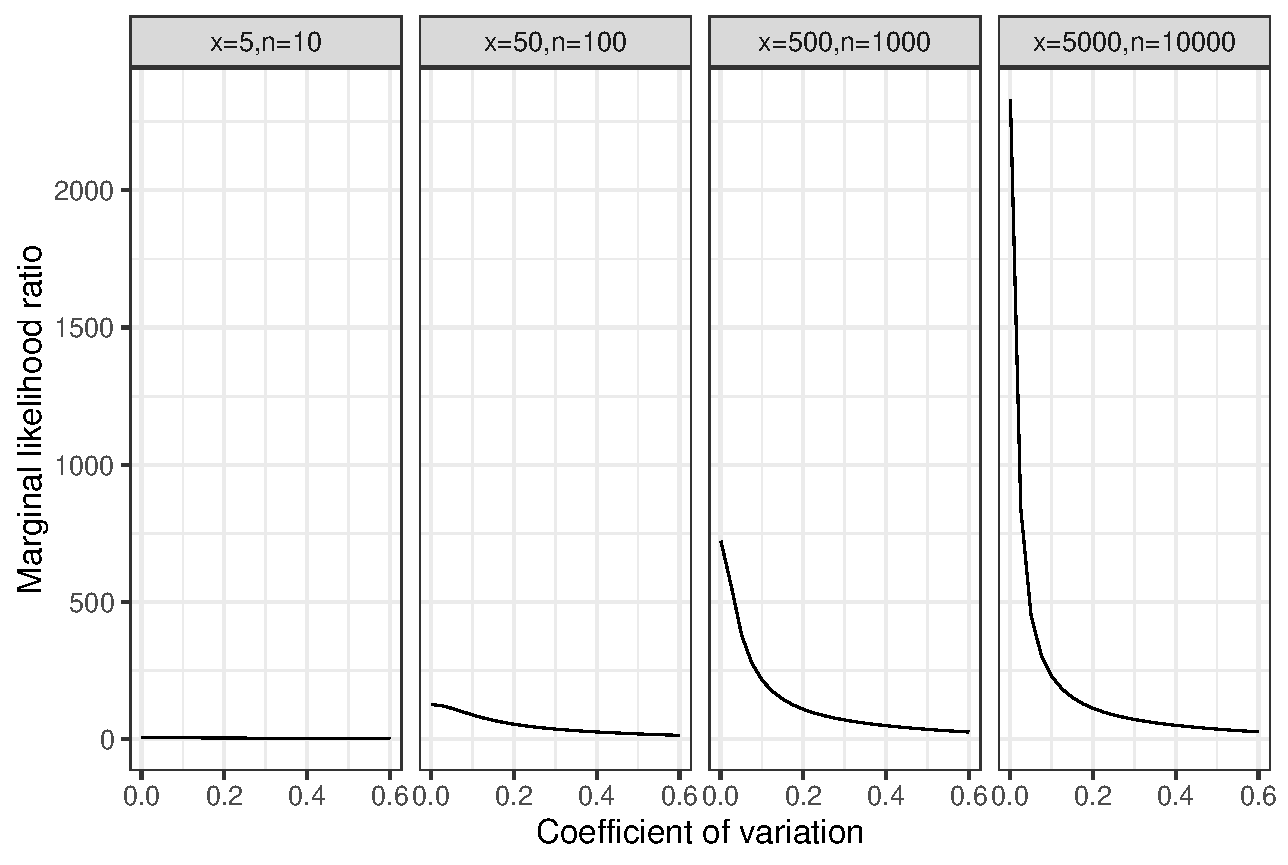
\includegraphics[scale=.45]{../plots/MaLs_ratios_oneCorrect.pdf}}
\subfigure[][Weights]{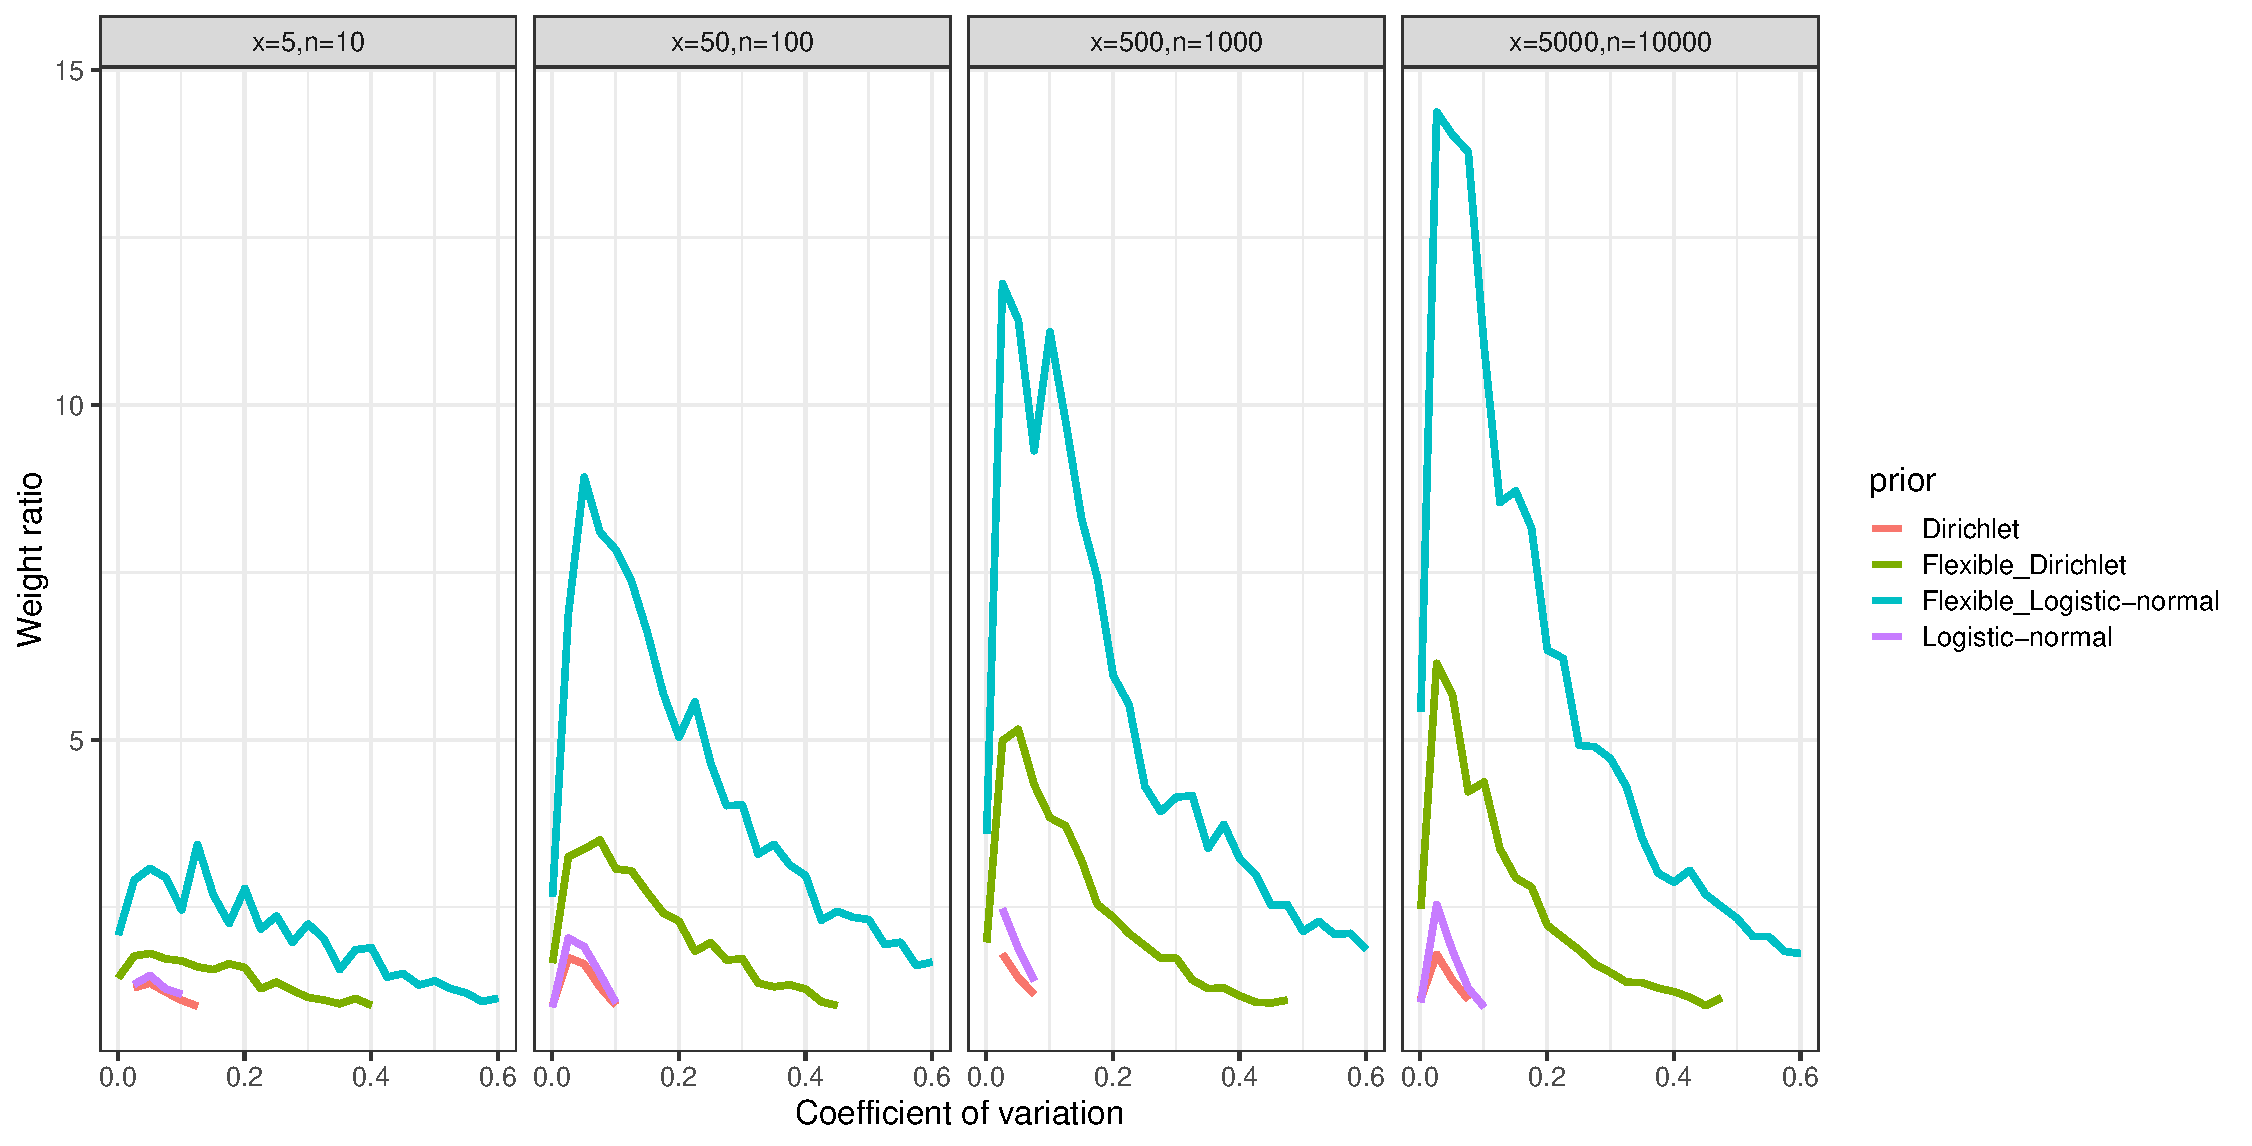
\includegraphics[scale=.45]{../plots/weight_ratios_oneCorrect.pdf}}
\end{center}
\caption{\textbf{Marginal likelihood and weight ratios for the simulated situation with one correct expert, various strengths of evidence}.
Panel (a) shows the ratio between the largest and second largest marginal likelihoods ($r_l$) as the correct expert's coefficient of variation ($c_2$) changes, while panel (b) shows the ratio between the largest and second largest posterior mean weights ($r_w$) in the same settings.
Vertical tiles show the observed data and colours in panel (b) show the hyperprior on $\boldsymbol\alpha$.
``Flexible'' priors are a Dirichlet(1/10, 1/10, 1/10, 1/10, 1/10) and the corresponding moment-matching logistic-normal.
We interrupt the lines for values of $c_2$ for which expert 2, the correct expert, does not attain the largest posterior weight (see text). 
}
\label{fig:one_correct_results}
\end{figure}

% \subsubsection{Two correct experts, different precisions}
% \label{sec:two_correct}
\subsection{Meta-analysis: HIV prevalence among MSM populations in Brazil}
\label{sec:metaAnalysis}

Another potential application of logarithmic pooling is in meta analysis.
Logarithmic pooling can also be used to combine probability distributions of a particular outcome estimated from several studies. 
In epidemiology, systematic review and meta analysis are popular tools for merging and contrasting results across multiple studies~\citep[Chapter 33]{Rothman2008}.
Moreover, estimation of disease prevalence and the effect of exposure variables are amongst the most important application of meta-analyses in epidemiology.
We illustrate the different approaches to assign weights in the logarithmic polling in the systematic review and meta analysis conducted by~\citet{Malta2010}. 
They analysed studies published from 1999 to 2009 assessing the HIV prevalence among men who have sex with another men (MSM) in Brazil. 
The authors have found six studies that estimated HIV prevalence in MSM population in Brazil. 
Data from each study consists of $n_i$ observed individuals, $y_i$ of which were infected with HIV.

Assuming a uniform prior for the HIV prevalence among MSM, denoted by $\varphi$, and a binomial model for each study, i.e. $Y_i \sim \text{Binomial}(n_i, \varphi)$. 
The posterior distribution for the HIV prevalence conditional on each study is then a Beta distribution with parameters $a_i = y_i + 1$ and $b_i = n_i - y_i + 1$, for $i=0,1, \ldots, 5$.
For the first part of our analysis of this problem we will assume $\boldsymbol F^{B}_\varphi$ to be composed of these posterior distributions.
In meta-analysis it is common for researchers to employ a Gaussian (normal) distribution instead of a distribution with support on $(0, 1)$, relying on the large sample normal approximation of the binomial distribution. 
Here we study how this choice of representation impacts the logarithmic pooling procedure by comparing the Beta and Gaussian distributions as representations of the HIV prevalence among MSM.

If the  probability density on $\varphi$ for each study is now
$$ f_i(\varphi; m_i, v_i) = \frac{1}{\sqrt{2\pi v_i}} \exp\left(\frac{-(\varphi-m_i)^2}{2v_i}\right), $$
where $m_i = y_i/n_i$ and $v_i = m_i(1-m_i)/n_i$.
We have
\begin{align}
\nonumber
\pi(\varphi)&= t(\boldsymbol\alpha)\prod_{i=0}^{K}f_i(\varphi; m_i, v_i)^{\alpha_i},\\
\nonumber
&\propto \prod_{i=0}^{K} \left[ \exp\left(\frac{-(\varphi-m_i)^2}{2v_i}\right) \right]^{\alpha_i},\\
&\propto \exp\left[-\frac{1}{2}\left\{\varphi\sum_{i=0}^K\frac{\alpha_i}{v_i} - 2\varphi\sum_{i=0}^K \frac{\alpha_im_i}{v_i} - \sum_{i=0}^K\frac{\alpha_im_i^2}{v_i} \right\}\right].
\end{align}
Completing the square shows $\pi(\varphi)$ is a normal distribution with parameters and $m^* = \frac{\sum_{i=0}^K w_im_i}{\sum_{i=0}^K w_i}$ and $v^* = [\sum_{i=0}^K w_i]^{-1}$,  where $w_i = \alpha_i/v_i$.
The entropy function is then:
\begin{equation}
 \label{eq:normalpoolentropy}
 H_{\pi}(\varphi) = \frac{1}{2}\left[ \ln(2\pi e) - \ln\sum_{i=0}^K w_i\right],
\end{equation}
which achieves its maximum when $\alpha_j = 1$ for $v_j = max(v_1, v_2, \ldots, v_K)$ and thus maximising entropy always leads to degenerate solutions.
The Kullback-Leibler divergence between the pooled distribution $\pi(\varphi)$ and each $f_i(\varphi)$ is then
\begin{equation}
 \label{eq:KL_Gaussian}
 \text{KL}( \pi || f_i) = \frac{1}{2}\log\left(\frac{v_i}{v^\star}\right) + \frac{v^\star + (m^\star - m_i)^2}{2v_i} - \frac{1}{2}.
\end{equation}
For the second part of our analysis of this example, we will assume that set of distributions to be combined, $\boldsymbol F^{G}_\varphi$, is composed by the Gaussian distributions described above.

Table \ref{tab:HIV_MSM} contains the sample size for each study, the total of HIV positive observed, and the estimated prevalence using the Beta distribution described above and a Gaussian distribution (see below). 
Note that the estimated prevalences among MSM are very high when compared with the HIV prevalence in the general population, 0.6\% \citep{Malta2010}.
In addition, there is considerable heterogeneity between studies, with (mean) estimates ranging from 6\%~\citep{Tun2008} to 24\%\citep{Sutmoller2002,Barcellos2003}.
\begin{table}[ht]
\caption{\textbf{Data extracted from the systematic review and meta analysis conducted by \citet{Malta2010} assessing the HIV prevalence among MSM in Brazil.}
$n_i$ is the sample size, $y_i$ is the total of HIV-positive participants in the $i$-th study.
Prevalence estimates are presented as mean and 95\% credibility intervals, either from a Beta distribution with parameters $a_i = y_i + 1$ and $b_i = n_i - y_i  +1$ or a Gaussian distribution with $m_i = y_i/n_i$ and $v_i = m_i(1-m_i)/n_i$ (see text).
}
\label{tab:HIV_MSM}
\centering
\begin{tabular}{rlrrcc}
  \hline
  & & & & \multicolumn{2}{c}{Estimated prevalence, $\varphi$ (95\% CI)}
\\
Study & Reference & $n$ & $y$ &  Beta & Gaussian \\ 
  \hline
0 & \cite{Tun2008}            &  658 &  44 & 0.068 (0.050--0.089) & 0.067 (0.048--0.086)\\ 
1 & \cite{Barcellos2003}  &  461 & 111 & 0.242 (0.204--0.282) & 0.241 (0.202--0.280)\\ 
2 & \cite{Carneiro2003} &  621 &  61 & 0.100 (0.077--0.124) & 0.098 (0.075--0.122)\\ 
3 & \cite{Sutmoller2002}       & 1165 & 281 & 0.242 (0.218--0.267) & 0.241 (0.217--0.266)\\ 
4 & \cite{BMH2000}                  &  642 &  57 & 0.090 (0.069--0.113) & 0.089 (0.067--0.111)\\ 
5 & \cite{Harrison1999}     &  849 &  99 & 0.118 (0.097--0.140) & 0.117 (0.095--0.138)\\ 
   \hline
\end{tabular}
\end{table}

In a meta-analytic context it also makes sense to consider giving weights to each study proportional to sample size, with larger studies receiving larger weights and hence more credence.
We have included this weighting, with $\alpha_i = n_i/ \sum_{i =0}^K n_i$, in our analysis, along with the maximum entropy and minimum KL solutions.
The weights obtained by maximising entropy and minimising KL divergence for both the Beta and Gaussian representations of the prevalence information are given in Table~\ref{tab:weights_MSM}.
While the maximum entropy method lead to the same degenerate solution for both distributions, giving all the weight to the study by~\cite{Barcellos2003}, minimising KL divergence lead to the studies by~\cite{Tun2008} and~\cite{Barcellos2003} being given non-zero weights.
Interestingly, while the minimum KL method for the Beta distribution representation lead to roughly equal weights, with the study by~\cite{Tun2008} being slightly favoured, the solution for the Gaussian representation assigned a much larger weight to the distribution from~\cite{Barcellos2003} (see Discussion).

\begin{table}[!ht]
\caption{\textbf{Weights obtained using different methods for the HIV prevalence example}.
Sample size pertains to assigning the  weights based on the normalised sample sizes ($\alpha_i = n_i/ \sum_{i =0}^K n_i$).
}
\centering
\begin{tabular}{cccccccc}
\hline
Method                            &    & $\alpha_0$ & $\alpha_1$ & $\alpha_2$ & $\alpha_3$ & $\alpha_4$ & $\alpha_5$ \\
\hline
\multirow{2}{*}{Maximum entropy} & Beta     & 0 & 1 & 0 & 0 & 0 & 0\\
                                  & Gaussian & 0 & 1 & 0 & 0 & 0 & 0\\
\multirow{2}{*}{Minimum KL divergence}      & Beta & 0.53 & 0.47 & 0 & 0 & 0 & 0 \\
                                  & Gaussian & 0.17 & 0.83 & 0 & 0 & 0 & 0\\
Sample size                      & & 0.15 & 0.11 & 0.14 & 0.27 & 0.15 & 0.19\\
\hline
\end{tabular}
\label{tab:weights_MSM}
\end{table}

Table~\ref{tab:prior_MSM} shows the estimates of the HIV prevalence among MSM in Brazil using different methods for obtaining the pooled distributions and Figure~\ref{fig:priors_pooled_MSM} shows the resulting densities.
For comparison, we also included results from the log-pooled distributions obtained with equal weights and the marginal prior on $\varphi$ induced by the Dirichlet (1/10, 1/10, 1/10, 1/10, 1/10, 1/10) and moment-matching logistic-normal priors on $\boldsymbol\alpha$. 
The heterogeneity observed across studies (Table~\ref{tab:HIV_MSM}) is also reflected in the variation in the combined (pooled) priors under different methods.
In contrast to the mean prevalence of $24\%$ yielded by the maximum entropy pooled prior, all other combined distributions have estimated mean prevalences in the range $[13\%, 16\%]$ for the Beta representation and $[12\%, 16\%]$ for the Gaussian representation.
As expected, the marginal priors for $\varphi$ induced by placing a prior on $\boldsymbol\alpha$ and then marginalising (\textit{via} Monte Carlo) yield broader distributions, which encompass the range of all original studies.
This effect is slightly more pronounced for the logistic-normal prior, pointing towards more flexibility compared to the Dirichlet.

\begin{figure}[!ht]
\begin{center}
\subfigure[][Study distributions]{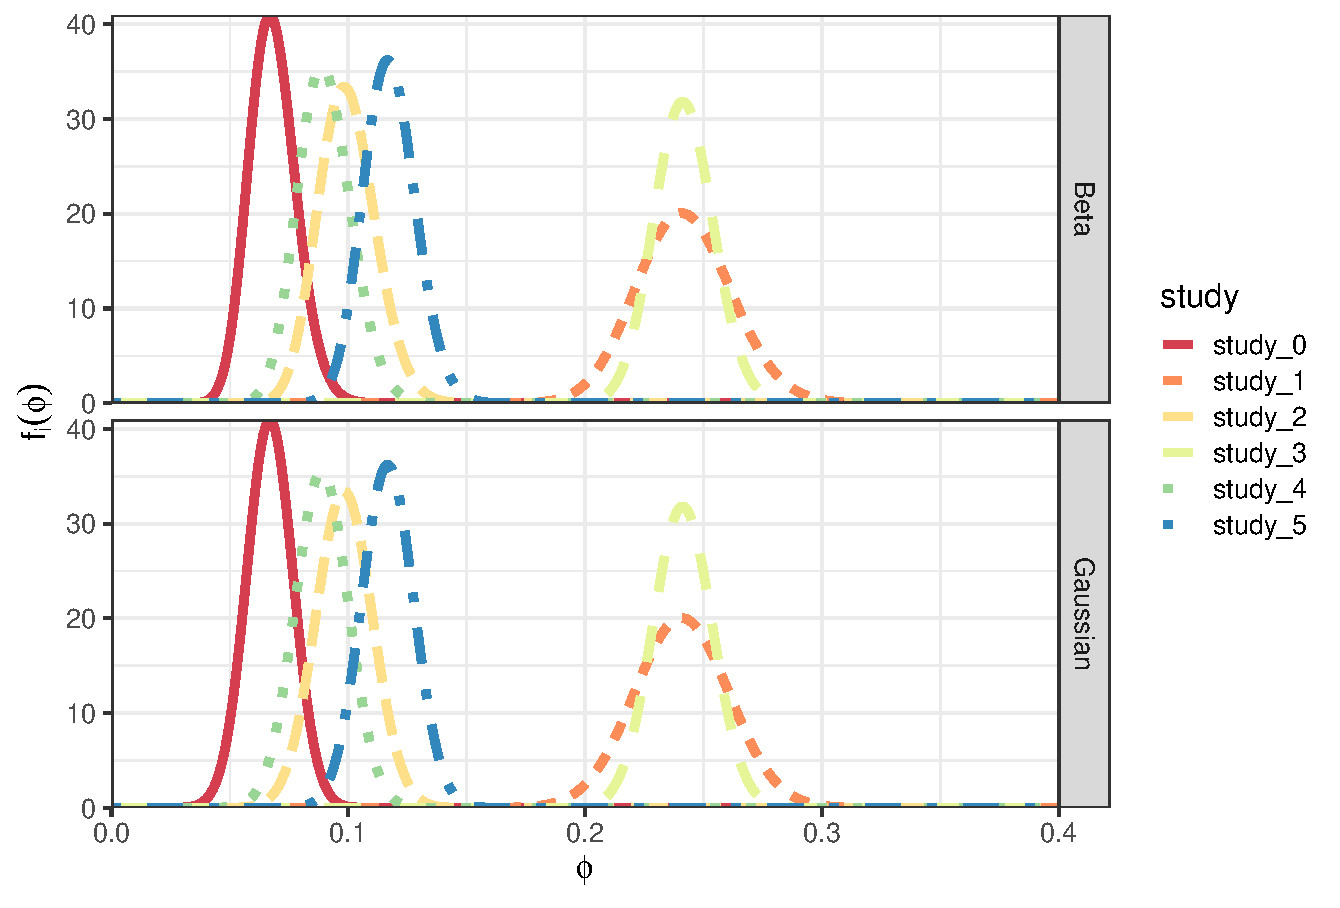
\includegraphics[scale=.45]{../plots/prior_densities_MSM.pdf}}
\subfigure[][Pooled distributions]{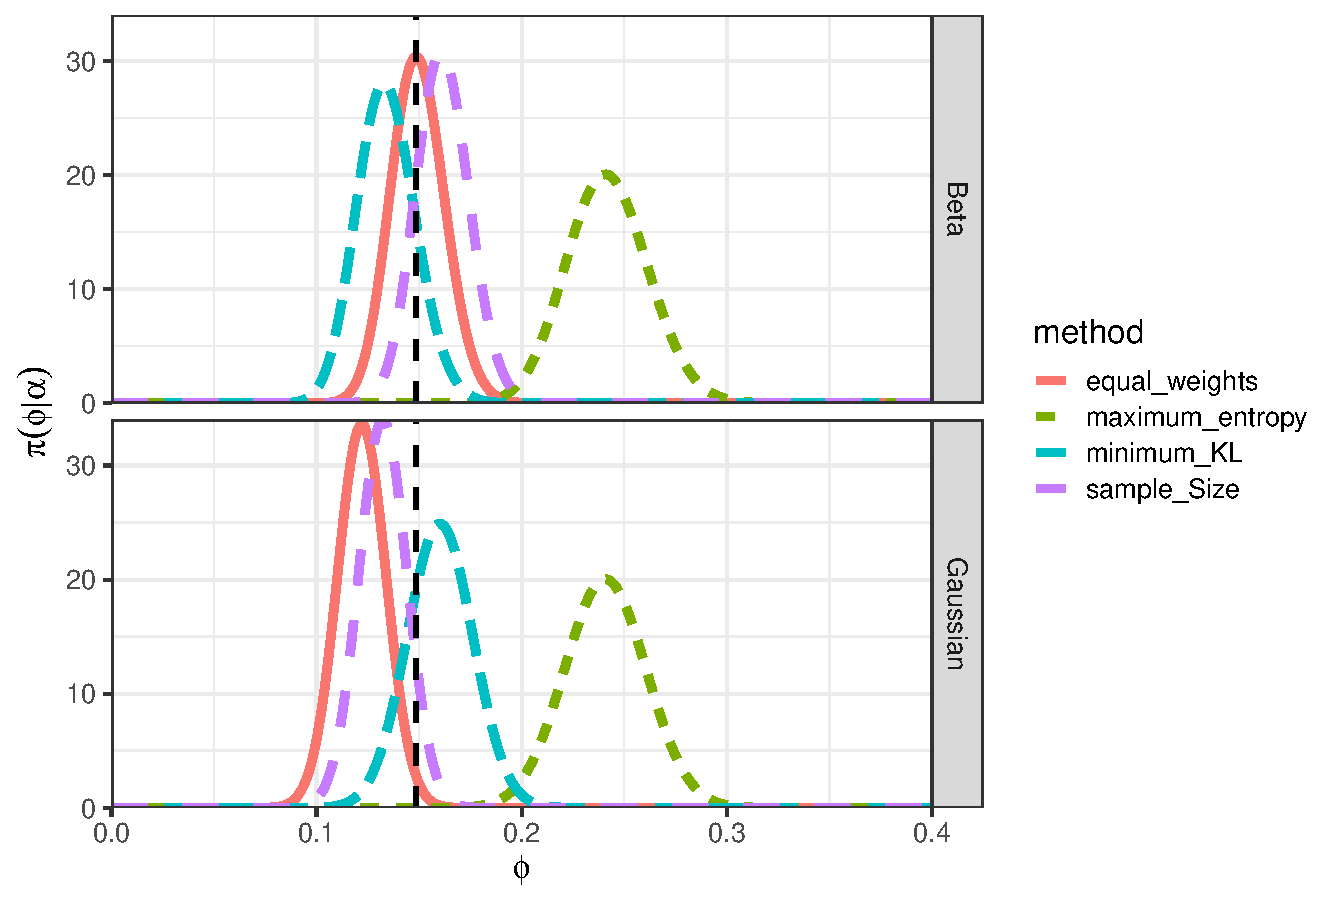
\includegraphics[scale=.45]{../plots/posterior_densities_MSM.pdf}}
\end{center}
\caption{\textbf{Densities for the HIV prevalence among MSM $\varphi$ using Beta and Gaussian distributions}.
Panel (a) shows the distributions obtained from  each study (see Table~\ref{tab:HIV_MSM}) and panel (b) shows the pooled distributions obtained using the methods discussed in this paper.
Vertical tiles show the distribution of choice (Beta or Gaussian) and the vertical dashed black line in panel (b) shows the estimate obtained by combining all studies, $\hat{\varphi} = \sum_{i = 0}^K y_i /\sum_{i = 0}^K n_i$.
}
\label{fig:priors_pooled_MSM}
\end{figure}

\begin{table}[ht]
\caption{\textbf{Mean and credibility intervals for each method for assigning the weights under two representations of information, HIV prevalence example.}
Sample size pertains to assigning the  weights based on the normalised sample sizes ($\alpha_i = n_i/ \sum_{i =0}^K n_i$).
}
\centering
\begin{tabular}{ccc}
 \hline
 & \multicolumn{2}{c}{Estimated HIV prevalence} \\
Method & Beta & Gaussian  \\ 
 \hline
 Equal weights &  0.150 (0.125--0.176)&  0.122 (0.099--0.145)\\ 
 Maximum entropy & 0.242 (0.204--0.282)  &  0.241 (0.202--0.280)\\ 
 Minimum KL  & 0.134 (0.107--0.163)  & 0.160 (0.129--0.192) \\ 
 Sample size & 0.162 (0.137--0.188) & 0.132 (0.109--0.155)\\
 Dirichlet prior & 0.144 (0.066--0.253) &  0.133 (0.063--0.250)\\ 
 Logistic-normal prior  & 0.143 (0.060--0.261) & 0.138 (0.059--0.259)\\ 
  \hline
\end{tabular}
\label{tab:prior_MSM}
\end{table}

\subsection{Bayesian melding with varying weights}
\label{sec:melding_apps}

In their seminal paper,~\cite{Poole2000} lay out the Bayesian melding as way to achieve full Bayesian inference for deterministic models -- see also Section~\ref{sec:background_melding} above.
In this section we explore two Bayesian melding applications and extend their approach by accommodating uncertainty about the weight $\alpha$ . 

\subsubsection{Bowhead whale population growth}
\label{sec:bowhead}

We begin with the analysis of a non-aged-structured population deterministic model (PDM) population model for bowhead whales originally carried out by~\cite{Poole2000}.
The model describes the annual population of bowhead whales in terms of the annual number of whales killed , $C_t$, the maximum sustainable yield rate (MSYR) and the initial bowhead population ($P_0$) as:
\begin{equation}
\label{eq:popmodel_bowhead}
 P_{t + 1} = P_t - C_t \times \text{MSYR} \times P_t \left( 1- (P_t/P_0)^2 \right).
\end{equation}
One of the quantities of interest in the model was $P_{\text{1993}}$, due to 1993 being the last year for which independent abundance measurements were available, allowing for model calibration.
Another important model quantity is the rate of population increase from 1978 to 1993, ROI, defined through
\begin{equation*}
 \label{eq:ROI_P1993}
P_{1993} = P_{1978}(1 + \text{ROI})^{15}. 
\end{equation*}
We are then interested in the model outputs $\phi = \{P_{1993}, \text{ROI}\}$.
The key idea is to account for the influence of the priors on the inputs $\theta = \{\text{MSYR}, P_0\}$ on $P_{1993}$ through the~\textbf{induced} distribution.
In particular, we aim at composing the prior distribution
\begin{equation}
 \label{eq:P1993_pool}
 \tilde{q}_{\Phi}(P_{1993}) \propto q_1^\ast(P_{1993})^\alpha q_2(P_{1993})^{1-\alpha},
\end{equation}
where $q_1^\ast$ is the induced distribution and $q_2$ is the natural prior on $P_{1993}$.
The main innovation we propose here is to place a probability distribution over $\alpha$ in order to relax the need to fix it to particular value.
We choose a $\text{Beta}(1, 1)$ prior as our $\pi_A$.
The target posterior is then 
\begin{equation}
 \label{eq:bowhead_posterior}
  p_{\Theta, M}(P_0, \text{MSYR}, \alpha \mid C_t) \propto \tilde{q}_{\Theta}(P_0, \text{MSYR}) L_1(P_0, \text{MSYR}) L_2(P_{1993})\pi_A(\alpha),
\end{equation}
where $\tilde{q}_{\Theta}$ is the suitably inverted distribution over the input space from the prior over the output space, $\tilde{q}_{\Phi}$ (see~\cite{Poole2000}, section 3.3.4). 
The subscript makes reference to the fact that this is a posterior over the inputs $\theta \in \Theta$ which are linked to the outputs $\phi \in \Phi$ by a deterministic model $M$, given by~(\ref{eq:popmodel_bowhead}).
Further details on priors and likelihoods are given in~\cite{Poole2000} and the Appendix of this paper.
We note that when $\alpha$ is random, it is important to include all of the normalising constants that depend on it~\citep{Neuenschwander2009}, in particular the normalising constant of the expression in (\ref{eq:P1993_pool}).

Here we will consider two ways of approximating (\ref{eq:bowhead_posterior}).
First, we used the sampling importance-resampling (SpIR) algorithm described in Section~\ref{sec:spIR}.
This method does not rely on any parametric approximation to the induced distribution $q_1^\ast$, instead using standard kernel methods to approximate the density at any point.
We used $k = l = 100, 000$ iterations to produce a sample from $p_{\Theta, M}$.
We also explored an HMC implementation in Stan.
However, for this implementation we needed to approximate $q_1^\ast$ by a parametric form.
Since $q_2$ is a normal distribution, we approximate $q_1^\ast$ by a normal distribution such that $\tilde{q}_{\Phi}$ (Equation~\ref{eq:P1993_pool}) can be written in closed-form.
We give further discussion on this choice in the Appendix.
Since $p_{\Theta, M}$ is a challenging target distribution, we used four independent chains of  $10,000$ iterations each.
We observed a low percentage of divergent iterations ($<$2\%), likely caused by the very challenging posterior geometry induced by high correlations between parameters.

In Figure~\ref{fig:bowhead_marginal_posteriors} we show the marginal posteriors for various quantities of interest, obtained with both algorithms and for fixed and varying $\alpha$.
As expected, SpIR are a bit noisier, but distributions are largely the same as obtained by MCMC.
For $\alpha$ in particular, despite the ruggedness of distribution obtained with SpIR, the mean and 95\% credibility intervals of both distributions match very closely: SpIR = 0.39 (0.02--0.87) and MCMC = 0.40 (0.02--0.91).
The high posterior uncertainty about $\alpha$ and the substantial overlap between distributions with fixed and varying $\alpha$ could be explained by the lack of sensitivity of the posterior distribution to $\alpha$.
We confirm this is indeed the case by running SpIR (original algorithm by~\cite{Poole2000}) for a few values of $\alpha$ (including the endpoints $0$ and $1$) and verifying very little difference in the resulting posteriors (Figure~\ref{sfig:alpha_sensitivity_bowhead}). 
\begin{figure}[!ht]
\begin{center}
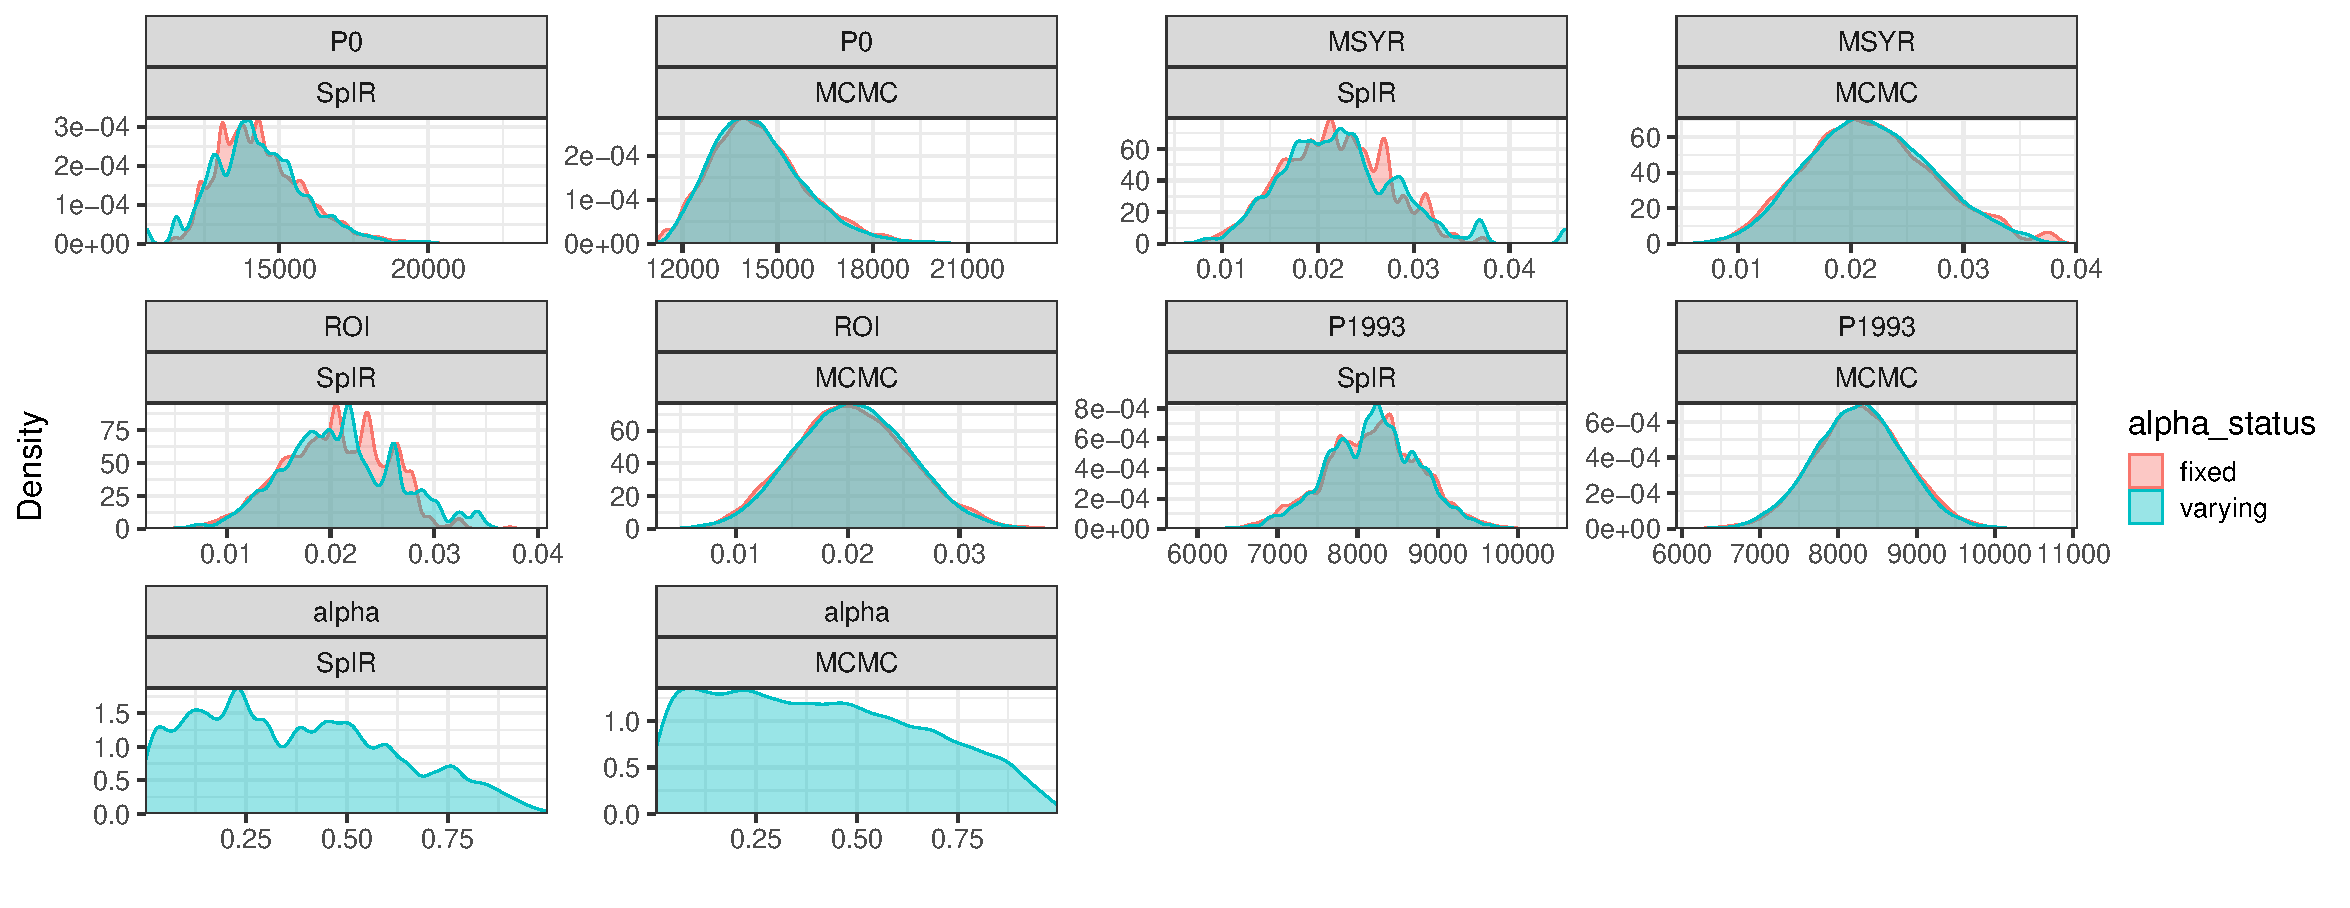
\includegraphics[scale=.45]{../plots/bowhead_posteriors.pdf}
\end{center}
\caption{\textbf{Marginal posterior distributions for various quantities of interest in the bowhead population model}.
We show the posterior distributions obtained by using sampling importance-resampling (SpIR) and Markov chain Monte Carlo (HMC-MCMC), for fixed $\alpha = 1/2$ and placing a prior $\pi_A$ on $\alpha$ (``varying'').
}
\label{fig:bowhead_marginal_posteriors}
\end{figure}

\subsubsection{Influenza in a boarding school}
\label{sec:SIR_flu}

Now, we will consider a deterministic epidemic model and how one can draw inference about a key epidemiological quantity, the basic reproductive number, $R_0$.
In 1978, an anonymous source reported an influenza H1N1 epidemic at a small boarding school in England~\citep{Anonymous1978}.
In total, 512 boys out of 763 became ill during the outbreak.
Due to the population being isolated and having high rates of contact, many of the assumptions of compartimental epidemic models hold.
In particular, the Susceptible-Infected-Removed (SIR) model is a good description of disease spread.
The model consists of the system of ordinary differential equations
\begin{eqnarray*}
\frac{dS}{dt}&=& - \beta SI,\\
\frac{dI}{dt}&=&  \beta SI - \gamma I,\\
\frac{dR}{dt}&=& \gamma I, 
\end{eqnarray*} 
where  $S(t) + I(t) + R(t) = 1 \: \forall t$, $\beta$ is the transmission (infection) rate and $\gamma$ is the recovery rate.
The basic reproductive number is 
\begin{equation}
\label{eq:r0def}
R_0 = \frac{\beta}{\gamma}. 
\end{equation}
The goal is to draw inference about $\beta$ and $\gamma$, and consequently about $R_0$, from data.
Data on the number of infected individuals per time ($Y(t)$) were obtained from the~\textbf{outbreaks} package~\citep{Outbreaks2019} and we choose to model the deviation from the ODE solution using log-normal errors, i.e.,
\begin{equation}
 \label{eq:log-normal_likelihood}
 L(Y(t)\mid \beta, \gamma, \sigma_I^2) = \text{log-normal}(\mu =  \log(I(t)), \sigma_I^2),
\end{equation}
where $I(t)$ is computed~\textit{via} an ODE solver.
Here we will consider a situation where one has priors on $\beta$ and $\gamma$, which induce a prior $q_1^\ast$ on $R_0$, and also a prior $q_2$ on $R_0$ directly.
This is the case when, for instance, one wants to make $q_2$ informative so as to incorporate expert knowledge and/or evidence from previous study.
For the priors on $\beta$ and $\alpha$ we choose commonly used, so-called ``uninformative'' log-normal priors with parameters $\mu_{\beta} = \mu_{\gamma} = 0$ and $\sigma_{\beta}^2 = \sigma_{\gamma}^2 = 1$, which induces a log-normal distribution ($q_1^\ast$) on $R_0$ with parameters $\mu_1 = \mu_\beta - \mu_\gamma$ and $\sigma_1^2 = \sigma_{\beta}^2 +  \sigma_{\gamma}^2$.
Using the extensive information gathered by~\cite{Biggerstaff2014}, we constructed an informative log-normal prior ($q_2$) with mean $1.5$ and variance $0.25^2$, which gives $\mu_2 = 0.3917656$ and variance $\sigma_2^2 =  0.1655264$.
This leads to a prior credibility interval of ($1.070$--$2.047$), which covers most of the estimates (and confidence intervals) of $R_0$ for Influenza found by~\cite{Biggerstaff2014}.
The target posterior is then
\begin{equation}
 \label{eq:target_SIR}
 p(\beta, \gamma, \alpha \mid Y(t)) \propto  L(Y(t)\mid \beta, \gamma, \sigma_I^2) q_1^\ast(R_0)^\alpha q_2(R_0)^{1-\alpha}\pi_A(\alpha),
\end{equation}
where we again let $\pi_A$ be a Beta(1,1) distribution.
This setup is convenient because it leads to a closed-form expression for the combined prior on $R_0$ (see Appendix, Section~\ref{sec:common_poolings}), while the log-normal priors are flexible and useful in practice.
We approximate the posterior in (\ref{eq:target_SIR}) using HMC as described above.

In Figure~\ref{fig:SIR_results}a we show the posterior distribution of the pooling weight $\alpha$, which favours high values with a mean and 95\% credibility interval of 0.77 (0.21--0.99).
The posterior distribution for $R_0$ obtained by letting $\alpha$ vary and also the resulting distributions of fixing $\alpha = 1/2$ or $\alpha = 1$ are shown in Figure~\ref{fig:SIR_results}b.
One can see that fixing $\alpha = 1$ and hence excluding the informative prior leads to a higher estimate of $R_0$ and fixing $\alpha = 1/2$ as per~\cite{Poole2000} leads to the lowest estimates.
The solution proposed in this paper, namely assigning $\alpha$ a prior and estimating it from data, leads to an intermediate solution.
Fixing $\alpha = 1/2$ also leads to underestimating the measured incidence (Figure~\ref{fig:SIR_results}c), whilst setting $\alpha = 1$ leads to mean predictions that are higher, albeit still underestimating the measured incidence.
Again, letting $\alpha$ vary leads to an intermediate solution.

\begin{figure}[!ht]
\begin{center}
\subfigure[][$\alpha$]{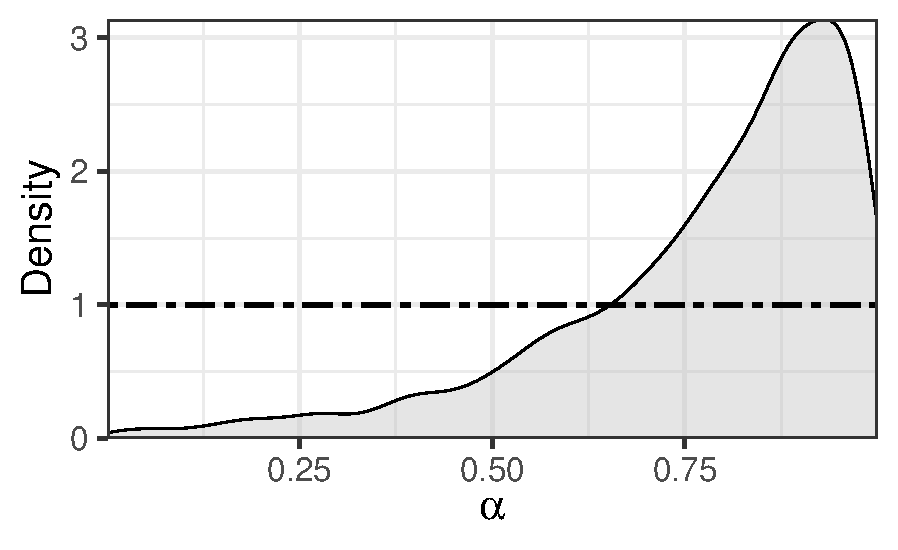
\includegraphics[scale=.35]{../plots/posterior_alpha_SIR_example.pdf}}
\subfigure[][$R_0$]{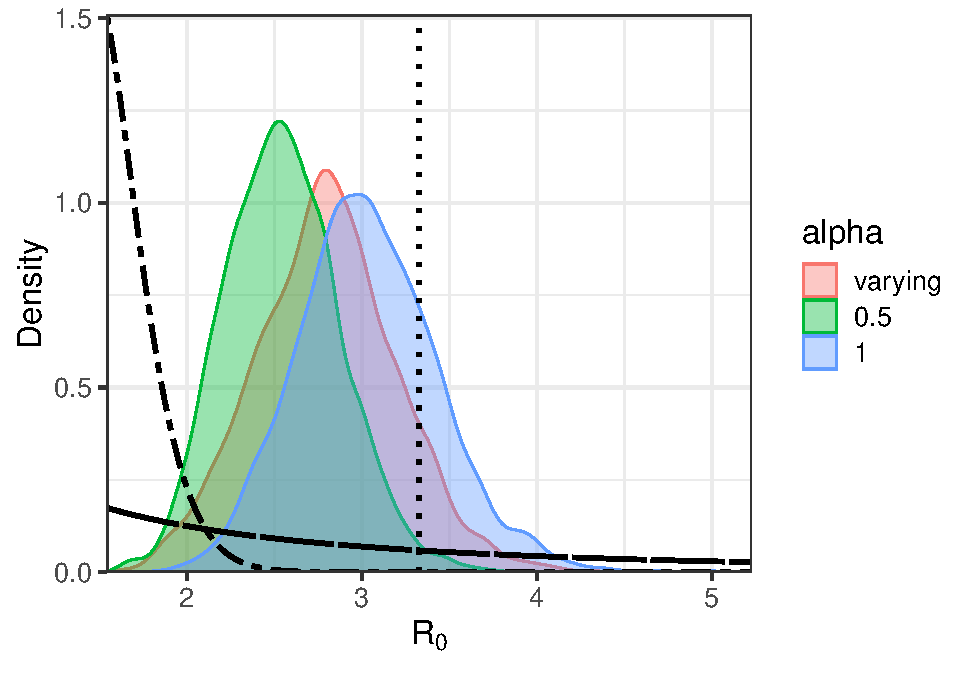
\includegraphics[scale=.35]{../plots/R0_posteriors_SIR_boardingSchool.pdf}}
\subfigure[][Predictions]{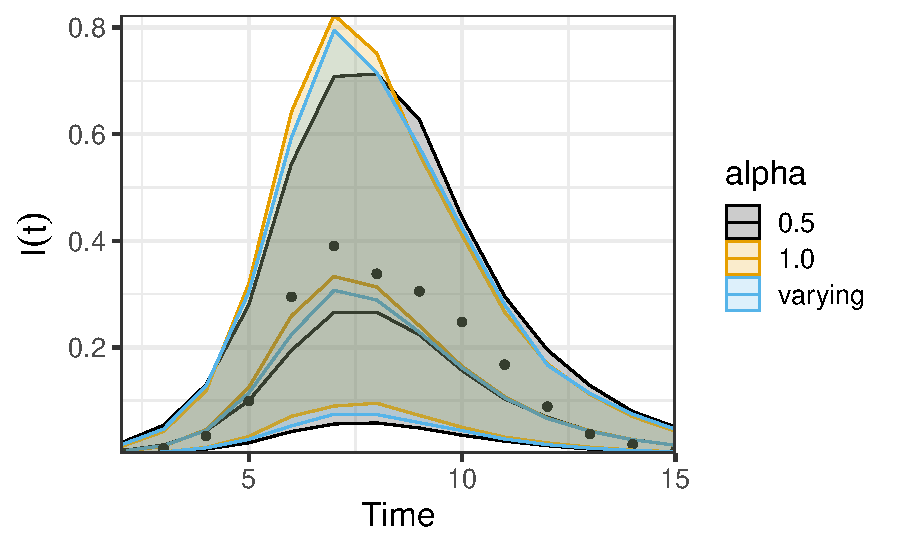
\includegraphics[scale=.45]{../plots/SIR_bands.pdf}}

\end{center}
\caption{\textbf{Estimates of the pooling weight ($\alpha$), the basic reproductive number ($R_0$) and predictions of the number of infected individuals}.
The posterior distribution for the pooling weight $\alpha$ is shown in panel (a), where the horizontal dashed line shows the prior density, a Beta(1, 1).
Panel (b) shows the posterior distribution for $R_0$ obtained with estimating $\alpha$ (``varying'') or fixing it to either $1/2$ or $1$.
Vertical line shows $R_0 = 3.78$~\citep{Murray2002}, the dot-dashed line shows the informative prior $q_2$ and the longdash line shows the induced prior $q_1^\ast$.
In panel (c) we show the posterior mean and 95\% credibility intervals for the proportion of infected individuals, again by either letting $\alpha$ vary or fixing it to either $1/2$ or $1$.
}
\label{fig:SIR_results}
\end{figure}

Our results agree somewhat with the estimate obtained by~\cite{Murray2002}, who finds $\rho = N/R_0 = 202$ and hence $R_0 = 3.78$, using purely numerical methods with no acknowledgement of uncertainty.
The highest estimates we obtained were for fixed $\alpha = 1$, $R_0$ = 3.02 (2.27--3.83).
This example showcases a desirable consequence of letting $\alpha$ vary: when the ``natural'' prior $q_2$, which is normally informative, is incompatible with the data, it will receive a lower weight ($\alpha$ closer 1) and hence allow the induced prior ($q_1$), which is usually more diffuse, to dominate.
In fact, as discussed by~\cite{Biggerstaff2014}, the spread of the 1978 boarding school epidemic is unusually fast when compared to regular seasonal Influenza and was likely caused by the lack of previous exposure of the population to the causing strain, H1N1.
The varying $\alpha$ approach makes it possible to deal with such an outlier data set by lowering the influence of the informative prior constructed based on previous studies.

\section{Discussion}
\label{sec:discussion}

First, we note that the properties in Section~\ref{sec:background} hold in more generality and the main choice of this paper, namely the choice to represent opinions as probability distributions, is not inconsequential.
As pointed out by~\cite{French1985}, one needs not assume that all experts express their opinion on the same scale.
This means one needs not assume that the expert opinions are encoded as probability distributions, let alone distributions in the same family.
Since our main goal is to motivate the use of logarithmic pooling in a statistical context, we argue this provides justification for the use of probability distributions.

With regard to the construction of the pooling weights ($\boldsymbol\alpha$) based on optimality criteria of the pooled distribution, we show that these usually lead to degenerate solutions that exclude one or more experts/information sources.
Considering the maximum entropy solutions in sections~\ref{sec:survivalProbs} and~\ref{sec:metaAnalysis} one might wonder whether maximising entropy can lead non-degenerate solutions.
A detailed characterisation of the conditions for the existence non-degenerate solutions is beyond the scope of the present paper, but we note that any configuration of the densities $\boldsymbol F_X$ can also lead to equally good (under the loss function) degenerate solutions, which is unavoidable due to the lack of a unique solution.
The minimum KL solutions (including the approach of~\citep{Rufo2012B}), which are unique, also lead to several experts being excluded.

Of course, one might argue that excluding a few or even all experts but one is not problematic since a few experts may, when suitably combined, summarise the information provided by the whole group.
The weights are not probabilities, but we argue that it would be preferable to have a solution that respects the so-called Cromwell's rule~\citep[pg. 91]{Lindley2013}, i.e., not assigning zero probability events that are logically impossible.
So far we have discussed approaches that consider only the information contained in the set of probability distributions $\boldsymbol F_X$.
But a hierarchical prior approach, which assigns a probability distribution to the weights, addresses both the issue of Cromwell's rule and the case where one has data $x$ from which the relative merits of the experts can be discerned by analysing the posterior distribution of $\boldsymbol\alpha$.
The results in Sections~\ref{sec:survivalProbs} and~\ref{sec:learning_rate} show that it is possible to learn the weights from data, while achieving efficient inference about the quantity of interest (but see below). 

The flexibility provided by the hierarchical prior deserves a bit more consideration.
For the Bayesian melding method, it is usual to set the pooling weight at $\alpha = 1/2$.
This choice leads to the so-called geometric pooling, since it is equivalent to taking the geometric mean of the densities $q_1^\ast$ and $q_2$ and is the only choice of $\alpha$ which is invariant to the re-labelling of inputs and outputs~\citep{Poole2000}.
Since there is usually clear scientific separation between inputs and outputs, we do not feel this is adequate justification for fixing the value of $\alpha$.
Indeed,~\cite{Poole2000} (Section 5.2) do argue that estimating $\alpha$ would be a fruitful path to explore and our results corroborate that view.
For the bowhead example (Section~\ref{sec:bowhead}), while the large posterior uncertainty about $\alpha$ precludes definitive statements, support for $\alpha < 1/2$ makes sense because $q_1^\ast$ is very diffuse.
By placing a lower weight on $q_1^\ast$, we favour $q_2$ as a prior for $P_{1993}$ and hence achieve a reduction  in posterior uncertainty, albeit a small one.
We obtained $\text{Pr}(\alpha < 1/2) = 0.69$ and $0.64$ for SpIR and MCMC, respectively.
In contrast, the SIR example (Section~\ref{sec:SIR_flu}) shows the situation in reverse, where the data are incompatible with the more informative prior.
The posterior distribution for $\alpha$ in this example accommodates this incompatibility, favouring the induced prior which results from non-informative priors on the inputs $\alpha$ and $\beta$.
For this example, $\text{Pr}(\alpha < 1/2)= 0.11$.

The use of logarithmic pooling is not without its pitfalls, however.
The meta-analysis in Section~\ref{sec:metaAnalysis} indicates that it can be very sensitive to the choice of distribution to represent expert opinion.
This is particularly true for the optimality-based methods, specially minimising KL distance.
Representing the distribution of HIV prevalence by a Beta or a Gaussian distribution lead to different studies being favoured by the minimum KL solution.
The (degenerate) maximum entropy solution was the same for both representations, but it is difficult to tell how dependent this is on the differences or lack thereof between Beta and Gaussian distributions due to the lack of uniqueness and propensity to achieve degenerate solutions.
The results in Section~\ref{sec:learning_rate} show that posterior inference for the weights only allows identifying the distribution most compatible with the data for some configurations of the set of opinions $\boldsymbol F_X$ (Figure~\ref{fig:one_correct_results}b).
More specifically, the ability to discern the ``best'' expert is linked to the separation between the expert opinions; if the ``correct'' expert provides a distribution that is too diffuse, we loose the ability to correctly identify it.
Importantly, of the four priors we considered here, only the logistic-normal prior with the first two moments matched to those of a Dirichlet(1/10, $\ldots$, 1/10) was flexible enough to allow correct identification over a large range of diffuseness.
Further research is needed in order to evaluate the possibility of more flexible priors.

As a final caveat, we note that if interest lies on a multivariate quantity $\theta \in \mathbb{R}^d$, $d>1$, obtaining the normalising constant $t(\boldsymbol\alpha)$ will entail computing a high-dimensional integral, which is unfeasible to do via quadrature and would likely necessitate specially-designed MCMC methods.

\section{Final remarks}
\label{sec:conclusion}

In this paper, our goal was to study how to one can assign the weights in logarithmic pooling such that it can be employed in statistical analysis.
We have shown how it can be a useful tool in constructing prior distributions, combining posterior distributions in meta-analysis and learning about the parameters of deterministic models.
We discussed how to approach the assigning of the weights based on optimality criteria such as maximum entropy and proposed a novel hierarchical prior approach that accommodates uncertainty about the weights and allows learning about them from data whilst providing more flexible prior modelling.
Future research will explore further applications of logarithmic pooling in statistical learning like for instance combining several posterior predictive distributions.
Work by~\cite{Johnson2018} and~\cite{Yao2018} has focused on generalising linear pools to combine probabilistic predictions, and logarithmic pooling could be explored as possibility that preserves characteristics such as log-concavity and relative propensity consistency.

Another interesting avenue for the future is studying the interaction between variable transformations and logarithmic pooling.
An example is a situation where one has distributions about a probability $p$ but is interested in the log-odds, $\omega = \log(p/(1-p))$.
Should the experts be judged by how reasonable their distributions look in transformed space?

In closing, we hope this paper showcases the usefulness -- and potential pitfalls -- of logarithmic pooling as a way of combining probability distributions and entices the statistical community to add it to their toolbox.


\section*{Acknowledgements}

The authors would like to thank Professors Adrian Raftery, Christian Genest and Mike West, as well as  Drs. David Poole and Felipe Figueiredo for helpful suggestions.
DAMV and LSB were supported in part by CAPES under CAPES/Cofecub project (N. 833/15).
FCC is grateful to Funda\c{c}\~ao Getulio Vargas for funding during this 
project.
This study was financed in part by the Coordenação de Aperfeiçoamento de Pessoal de Nível Superior - Brasil (CAPES) Finance Code 001.
LMC was partially supported by a postodoctoral fellowship from CAPES.
% {\footnotesize
\bibliography{pooling}
% }

\newpage 

\appendix
\section{Appendix}
\renewcommand\thefigure{S\arabic{figure}}    
\setcounter{figure}{0} 

\subsection{Proofs}

Here we provide a simple proof of Theorem~\ref{thm:normalisation} using H\"{o}lder's inequality.
\begin{proof}
We begin by noting that $\pi(\theta)$ can be re-written as:
\begin{equation}
\label{eq:pirewritten}
 \pi(\theta) \propto f_0(\theta)\prod_{j=1}^{K} \left(\frac{f_j(\theta)}{f_0(\theta)}\right)^{\alpha_j}.
\end{equation}
Let $X_j = \frac{f_j(\theta)}{f_0(\theta)}, j=1, 2,\ldots, K$. 
Then, integrating the expression in (\ref{eq:pirewritten}) is equivalent to finding 
\begin{equation}
\label{eq:expectations}
\mathbb{E}_{0}\left[\prod_{j=1}^KX_j^{\alpha_j}\right] \leq \prod_{j=1}^K \mathbb{E}_{0}[X_j]^{\alpha_j},
\end{equation}
where $\mathbb{E}_{0}[\cdot]$ is the expectation w.r.t $f_0$ and (\ref{eq:expectations}) follows from H\"{o}lder's inequality for expectations~\citep{Yeh2011}.
Since $\forall j$ we have $\mathbb{E}_{0}[X_j]^{\alpha_j} = \left(\int_{\boldsymbol\Theta}f_0(\theta)\frac{f_j(\theta)}{f_0(\theta)}\, d\theta\right)^{\alpha_j}=1^{\alpha_j}$, Theorem~\ref{thm:normalisation} is proven.
\end{proof}

To establish Theorem~\ref{thm:concavity}, we will need the following result from~\cite{Genest1984}.
\begin{lemma}
\label{lem:RPC_representation}
\textbf{Representation of a pooling operator with RPC}~\citep[eq. 3.1]{Genest1984}.
The \underline{only} relative propensity consistent operator can \underline{always} be represented by
\[ \mathcal{T} \left( \boldsymbol F_\theta \right)(\theta) = \boldsymbol B\left( \boldsymbol F_\theta \right) c(\theta) \prod_{i=0}^K \left[f_i(\theta) \right]^{w_i},\]
with $\boldsymbol B\left( \boldsymbol F_\theta \right) > 0$, $c(\theta) >0$  and $\alpha_0, \alpha_1, \ldots, \alpha_K \geq 0$ arbitrary. 
\end{lemma}
We refer the reader to~\cite{Genest1984} for the proof.
Now we can state the proof of Theorem~\ref{thm:concavity}.
\begin{proof}
First, we will show by direct calculation that logarithmic pooling (LP) leads to a log-concave distribution.
Notice that each $f_i$ can be written as $ f_i(\theta) \propto e^{\nu_i(\theta)}$, where $\nu_i(\cdot)$ is a concave function.
We can then write
\begin{align*}
 \pi(\theta \mid \boldsymbol \alpha) &\propto \prod_{i=0}^{K} [\exp(\nu_i(\theta))]^{\alpha_i},\\
             &\propto \exp(\nu^{\ast}(\theta)),
\end{align*}
 where $\nu^{\ast}(\theta) = \sum_{i=0}^{K}\alpha_i\nu_i(\theta)$ is a concave function because it is a linear combination of concave functions.
 
We will now show that LP is the only operator that guarantees log-concavity when $\boldsymbol F_\theta$ is a set of concave distributions.
First, recall that LP is the only pooling operator that enjoys RPC (Remark~\ref{rmk:properties_RPC}).
With the goal of obtaining a contradiction, suppose that there exists a pooling operator $\mathcal{T}$ that is log-concave but does not enjoy RPC.
 From Lemma~\ref{lem:RPC_representation}, we know that, under this assumption, $\mathcal{T}$ cannot be written in the form $\boldsymbol B(\boldsymbol F_\theta) c(\theta) \prod_{i=0}^K f_i(\theta)^{\alpha_i} $.
But every non-negative log-concave function $g(\theta)$ can be represented as
 \begin{equation}
 \label{eq:lc_rep}
  g(\theta) = a \cdot c(\theta) \cdot h(\theta),
 \end{equation}
with $a \geq 0$ and $c(\theta)$ and $h(\theta)$ non-negative and log-concave, but otherwise arbitrary.
Under the assumptions on $\boldsymbol F_\theta$, we have that $h(\theta) := \prod_{i=0}^K f_i(\theta)^{\alpha_i}$ is non-negative and log-concave.
Since $c(\theta)$ is bound to be positive, it may very well be (log-)concave.
Therefore $\mathcal{T}$ can in fact be represented in the form of Lemma~\ref{lem:RPC_representation}, contradicting our initial assumption that $\mathcal{T}$ can at same time be log-concave but not enjoy RPC.  
\end{proof}

Now we move on to the exponential family results in Section~\ref{sec:expofamily}.
To see that equation~(\ref{eq:entropypriorEF}) holds:
\begin{eqnarray*} 
H_\pi(\theta) & = & \mathbb{E}[-\log(\pi(\theta)], \\
              & = & - \int \log(\pi(\theta)) \pi(\theta) \, d\theta, \\
              & = & - \int (\log(K(a^*, b^*) + \theta a^* - s(\theta) b^*) \pi(\theta) \, d\theta, \\
              & = & - \log(K(a^*, b^*)) - a^*  \mathbb{E}[\theta] +  b^*  \mathbb{E}[s(\theta)].
\end{eqnarray*}
Likewise for equation~(\ref{eq:KLpriorEF}), we have 
\begin{eqnarray*} 
KL(f_i || \pi) & = & \mathbb{E}_\pi[\log(f_i(\theta)-\log(\pi(\theta)], \\
              & = & \int [\log( K(a_i,b_i) e^{\theta a_i - b_i s(\theta)}) - \log(K(a^*,b^*) e^{\theta a^* - b^* s(\theta)}) ] \pi(\theta) \, d\theta, \\
              & = & \int [\log( K(a_i,b_i)) - \log(K(a^*,b^*)) + (a_i - a^*) \theta  - (b_i - b^*) s(\theta) \pi(\theta) \, d\theta, \\
              & = & \log( K(a_i,b_i)) - \log(K(a^*,b^*)) + (a_i - a^*) \mathbb{E}_\pi[\theta] - (b_i - b^*) \mathbb{E}_\pi[s(\theta)]. 
\end{eqnarray*}

\newpage
\subsection{Bowhead population growth model: details}

For convenience, here we will describe the priors and likelihoods used by~\cite{Poole2000} in their analysis of the bowhead whale population model, as well as some of our modelling choices.
For $P_0$ only a shifted gamma prior is available, i.e.,
\begin{equation*}
 q(P_0) = \frac{b_{P_0}^{a_{P_0}}}{\Gamma(a_{P_0})} (P_0 - s_{P_0})^{a_{P_0}-1} \exp\left(-b_{P_0}(P_0 - s_{P_0})\right), \: P_0 > s_{P_0},
\end{equation*}
with $s_{P_0} = 6400$, $a_{P_0} = 2.8085$ and $b_{P_0} = 0.0002886$.
The maximum sustainable yield rate (MSYR) is assigned Gamma prior with parameters $a_{\text{MSYR}} = 8.2$ and $a_{\text{MSYR}} = 372.7$.

The size of the bowhead population in 1993, $P_{1993}$, is an output of the model for which there are both a prior and a likelihood.
The prior ($q_2$) is a Gaussian distribution with mean $\mu_{1993} = 7800$ and standard deviation $\sigma_{1993} = 1300$, while the likelihood ($L_2$) is also a Gaussian distribution but with mean $\mu_{1993}^\prime = 8293$ and standard deviation $\sigma_{1993}^\prime = 626$.
For the rate of increase (ROI),~\cite{Poole2000} use a likelihood that is proportional to  $\exp(a + b \times t_8) - 1$, with $a = 0.0302$ and $b = 0.0068$ where $t_8$ is a random variable with Student t distribution with $\nu = 8$ degrees of freedom.
This leads to the density
\begin{equation*}
 L(\text{ROI} \mid \nu, a, b) = \frac{\Gamma((\nu + 1)/2)}{\Gamma(\nu/2)}\frac{1}{\sqrt{\nu\pi}} \left( 1 + \left((\log(\text{ROI} + 1) - a)/b\right)^2 \right)^{-(\nu+ 1)/2}\frac{1}{|b(\text{ROI} + 1)|},\: \text{ROI} > -1.
\end{equation*}

For the Stan implementation, we approximate the distribution induced on $P_{1993}$ by the prior on $P_0$ and $\text{MSYR}$ and transformation in~(\ref{eq:popmodel_bowhead}), $q_1^\ast$,  by a normal distribution with mean $\mu_{\text{ind}} = 18137.70$ and standard deviation $\sigma_{\text{ind}} = 6146.85$ .
This step deserves a bit more consideration.
As discussed by~\cite{Poole2000}, $q_1^\ast$ is very diffuse and likely has heavier tails than a normal distribution.
Hence it would make sense also to consider the skew-normal and log-normal families as approximating distributions.
On the other hand, we note that approximating $q_1^\ast$ with a normal distribution allows closed-form computation of the coherised prior $\tilde{q}_{\Phi}(P_{1993})$.
In Figure~\ref{sfig:induced_P1993} we show the densities of a normal, skew-normal and log-normal distributions fitted to $100, 000$ simulations from $q_1^\ast$ by maximum likelihood.
While the skew-normal provides better fit (AIC: 1150814) we do not feel the difference in fit to the normal (AIC: 1152288) justifies the increased technical overhead of not being able to compute the coherised prior in closed-form.
Both distributions provide much superior fit than the log-normal (AIC: 1181753).

\begin{figure}[!ht]
\begin{center}
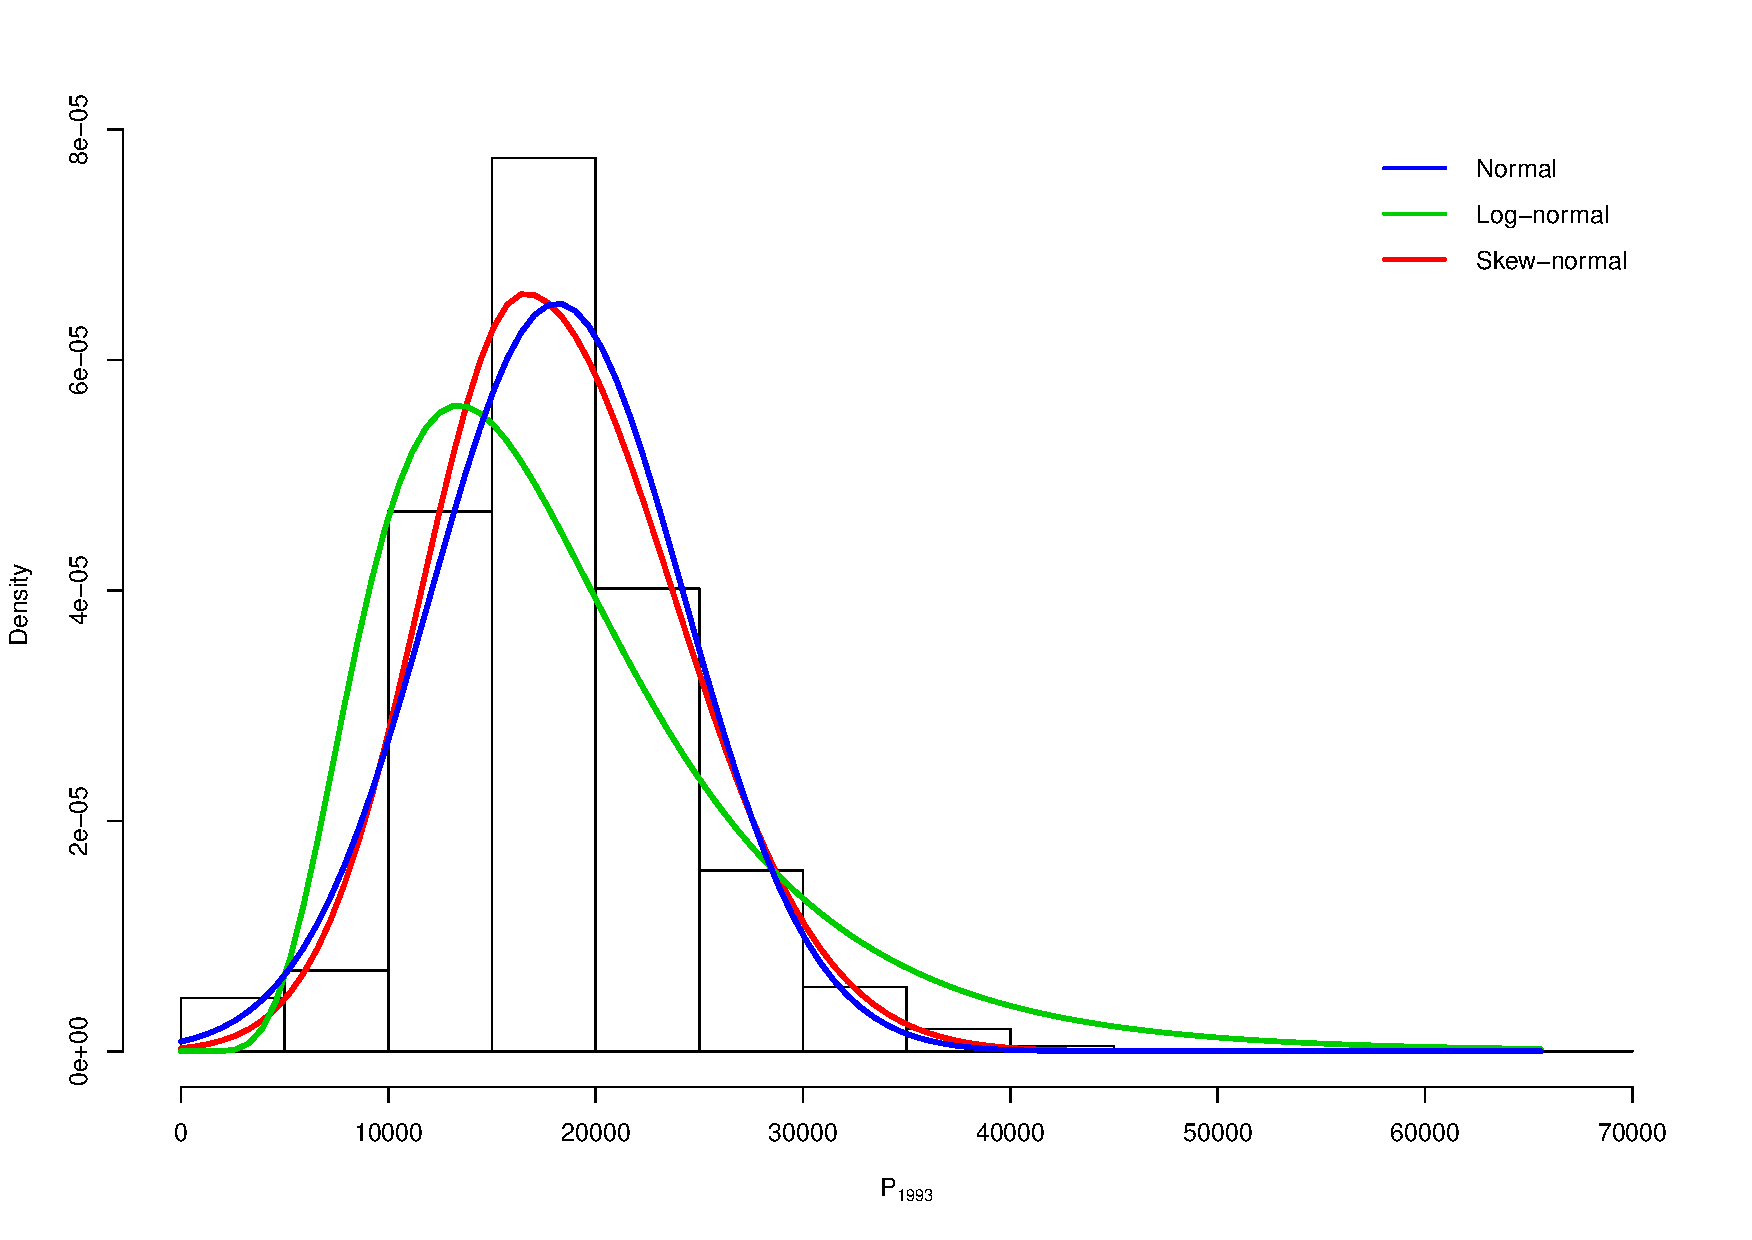
\includegraphics[scale=.5]{../plots/induced_P1993.pdf}
\end{center}
\caption{\textbf{Induced distribution on $P_1993$ ($q_1^\ast$) and approximating distributions}.
We present the histogram of $100, 000$ simulations from the prior.
Lines show the densities of the three distributions considered.
}
\label{sfig:induced_P1993}
\end{figure}

Note that the sampling-importance-resampling discussed in Section~\ref{sec:spIR} does not necessitate any parametric approximation, employing a density estimation method instead.

In Figure~\ref{sfig:alpha_sensitivity_bowhead} we show the posterior distributions obtained with different values of $\alpha$ using SpIR.
\begin{figure}[!ht]
\begin{center}
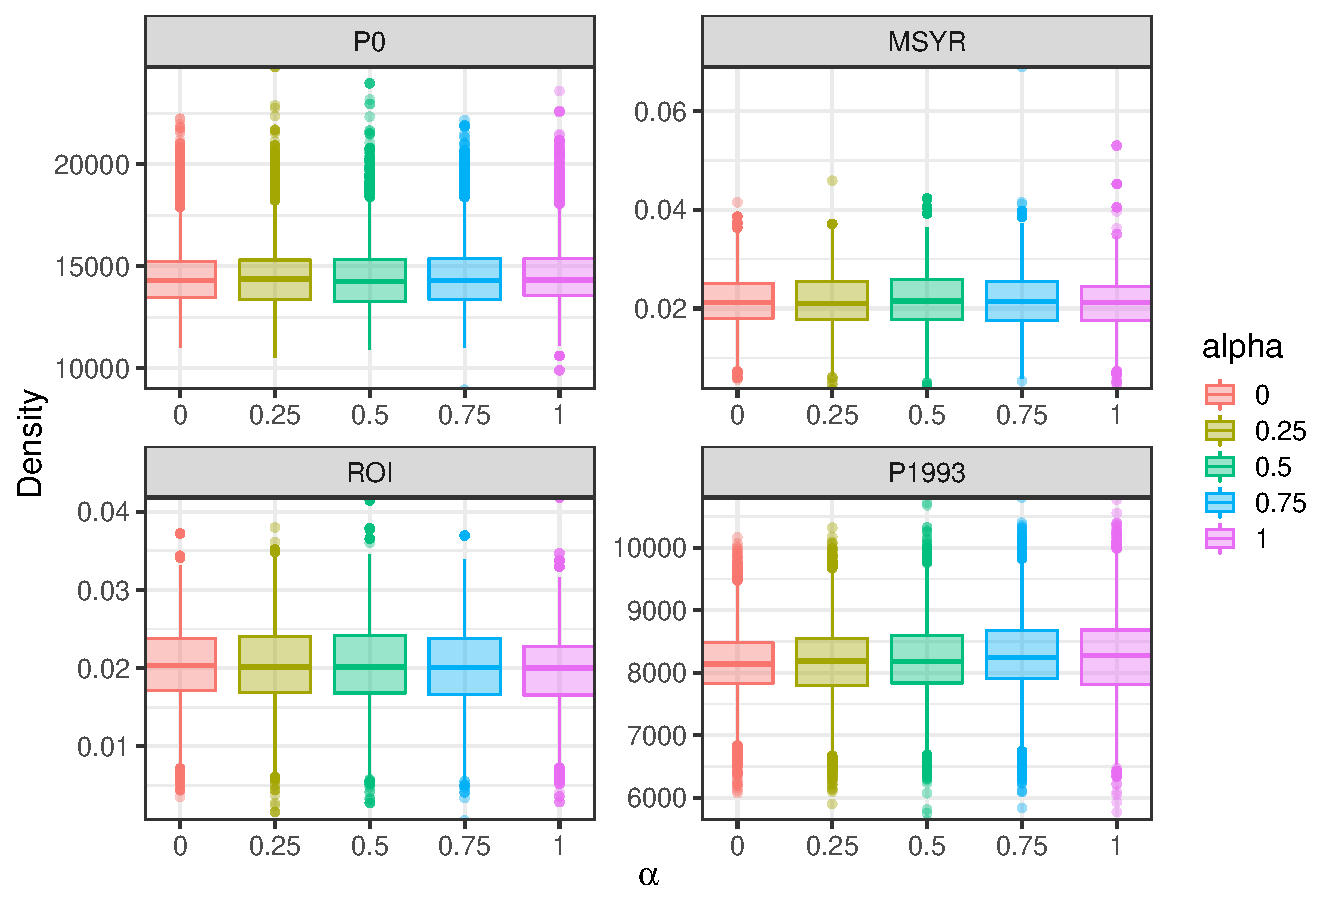
\includegraphics[scale=.65]{../plots/alpha_sensitivity_bowhead.pdf}
\end{center}
\caption{\textbf{Sensitivity of posterior inferences to varying the value of $\alpha$, bowhead population model}.
}
We show the posterior distributions obtained by SpIR for $P_0$, MSYR, ROI and $P_1993$ as we fix $\alpha$ to different values.
\label{sfig:alpha_sensitivity_bowhead}
\end{figure}

\newpage
\subsection{Pooling of common distributions}
\label{sec:common_poolings}

In the main text we give the pooled distributions if one assumes a set of Beta (Section~\ref{sec:survivalProbs}) or Gaussian (Section~\ref{sec:metaAnalysis}) distributions as the expert opinions.
In this section we give further results for the pooling of commonly used distributions.

\subsubsection{Gamma}
\label{sec:gamma}
Suppose $K + 1$ experts are called upon to elicit prior distributions for a quantity $\lambda \in \mathbb{R}^+$.
A convenient parametric choice for $\mathbf{F}_\lambda$ is the Gamma family of distributions, for which densities are of the form
$$ f_i(\lambda;a_i,b_i) = \frac{b_i^{a_i}}{\Gamma(a_i)} \lambda^{a_i-1} e^{-b_i\lambda}.$$
The log-pooled prior $\pi(\lambda)$ is then
\begin{align}
\nonumber
\pi(\lambda)&= t(\boldsymbol\alpha)\prod_{i=0}^{K}f_i(\lambda;a_i,b_i)^{\alpha_i},\\
\nonumber
&\propto \prod_{i=0}^{K} \left(\lambda^{a_i-1} e^{-b_i\lambda}\right)^{\alpha_i},\\
\label{eq:gammapois}
&\propto \lambda^{a^*-1} e^{-b^*\lambda},
\end{align}
where $a^* =\sum_{i=0}^{K}\alpha_ia_i$ and $b^* = \sum_{i=0}^{K}\alpha_ib_i$.
Noticing (\ref{eq:gammapois}) is the kernel of a gamma distribution with parameters $a^*$ and $b^*$, $H_{\pi}(\lambda)$ becomes
\begin{equation}
\label{eq:entropygamma}
H_{\pi}(\lambda; \boldsymbol\alpha) = a^* - \log b^* + \log \Gamma(a^*) + (1-a^*)\psi(a^*),
\end{equation}
where $\psi(\cdot)$ is the digamma function.
The Kullback-Liebler divergence between the pooled density $\pi$ and each density is:
\begin{equation}
 \label{eq:KLgamma}
 \text{KL}(\pi || f_i) = (a_i-a^*)\psi(a_i) - \log\Gamma(a_i) + \log\Gamma(a^*) + a^*\left(\log\frac{b_i}{b^*}\right) + \frac{a_i}{b_i}(b^*-b_i).
\end{equation}

\subsubsection{Log-normal} 
\label{sec:log-normal}
Another popular choice for modelling a quantity $\eta \in \mathbb{R}^+$ is the log-normal family.
Following the results given in Section~\ref{sec:metaAnalysis}, we know that the pool of log-normal distributions with parameters $\mu_i$ and $\sigma_i^2$ is a log-normal distribution with parameters $\mu^\star = \frac{\sum_{i=0}^K w_im_i}{\sum_{i=0}^K w_i}$ and ${\sigma^\star}^2 = [\sum_{i=0}^K w_i]^{-1}$,  where $w_i = \alpha_i/\sigma_i^2$.

The entropy function is then:
\begin{align}
 \nonumber
 H_{\pi}(\eta ; \boldsymbol\alpha) &= \log_2(e)\log\left(\sigma^\star\exp\left(\mu^\star + \frac{1}{2}\right) \sqrt{2\pi}\right),\\
 \label{eq:log-normalpoolentropy}
 & = \log_2(e) \left[\log\left(\sigma^\star\right) +  \mu^\star + \frac{1}{2} + \log(\sqrt{2\pi})\right].
\end{align}

The KL divergence evaluates to
\begin{equation}
 \label{eq:KL_log-normal}
 \text{KL}(\pi || f_i) = \frac{1}{2\sigma_i^2} \left[ \left( \mu^\star - \mu_i \right)^2 + {\sigma^\star}^2 - \sigma_i^2 \right] + \log\left(\frac{\sigma_i^2}{{\sigma^\star}^2}\right).
\end{equation}


\subsubsection{Poisson}
\label{sec:poisson}

If the quantity of interest is a count $y = 0, 1, \ldots, $ and $\boldsymbol F_y$ is a set of Poisson distributions with rate parameters $\boldsymbol\lambda = \{\lambda_0, \lambda_1, \ldots, \lambda_K \}$.
We have 
\begin{align}
\nonumber
 \pi(y) &\propto \prod_{i = 0}^K \left(\frac{\lambda_i^y}{y!}\right)^{\alpha_i},\\
 \label{eq:pooled_Poisson}
 \pi(y) &= \frac{\exp(-\lambda^\star) {\lambda^\star}^{y}}{y!},\: \text{with}\: \lambda^\star = \prod_{i = 0}^K \lambda_i^{\alpha_i}.
 \end{align}
The entropy of the pooled distribution is 
\begin{equation}
 \label{eq:entropy_Poisson}
 H_\pi(y; \boldsymbol\alpha) = -\lambda^\star \log\left(\frac{\lambda^\star}{e}\right) + E_\pi\left[ \log(k!) \right],
\end{equation}
where the latter term cannot be evaluated in closed-form, but efficient approximations exist~\citep{Evans1988}.

The KL divergence is
\begin{align}
 \nonumber 
 \text{KL}(\pi || f_i) &= \lambda^\star \log\left( \frac{\lambda^\star}{\lambda_i} \right) + \lambda_i - \lambda^\star,\\
 \label{eq:KL_Poisson}
 & = \lambda^\star \left[ \sum_{k = 0}^K \alpha_k \log(\lambda_k) - \log(\lambda_i) \right] + \lambda_i - \lambda^\star.
\end{align}

\end{document} 
